\documentclass{article}

% LaTeX packages
\usepackage{algorithm}
\usepackage[algo2e, vlined, ruled, noend]{algorithm2e}
\usepackage{algorithmic}
\usepackage{amsmath}
\usepackage{amssymb}
\usepackage{amsthm}
\usepackage[english]{babel}
\usepackage[singlelinecheck=false]{caption}
\usepackage[colorlinks=true,citecolor=blue,linkcolor=blue]{hyperref}
\usepackage{natbib}
\usepackage{thmtools}
\usepackage{tikz}
\usepackage{color}
\usepackage{comment}
\usepackage{commath}
\usepackage{dsfont}
\usepackage{framed}
\usepackage{caption, subcaption}
\usepackage{authblk}
\usepackage{fullpage}
\usepackage{times}
%\usepackage{icml2019}  % anonymous submission
%\usepackage[accepted]{icml2019}  % camera ready version
\usepackage[outdir=./]{epstopdf}
% TikZ packages
\usetikzlibrary{arrows}
\usetikzlibrary{angles}
\usetikzlibrary{backgrounds}
\usetikzlibrary{calc}
\usetikzlibrary{cd}  % commutative diagrams
\usetikzlibrary{decorations.markings}
\usetikzlibrary{intersections}
\usetikzlibrary{patterns}
\usetikzlibrary{shapes}
\usetikzlibrary{through}

% Math environments
\newtheorem{definition}{Definition}
\newtheorem{proposition}[definition]{Proposition}
\newtheorem{lemma}[definition]{Lemma}
\newtheorem{theorem}[definition]{Theorem}
\newtheorem{corollary}[definition]{Corollary}

% Math symbols and commands
\newcommand{\calB}{\mathcal{B}}
\newcommand{\calA}{\mathcal{A}}
\newcommand{\calF}{\mathcal{F}}
\newcommand{\calH}{\mathcal{H}}
\newcommand{\one}{\mathds{1}}
\newcommand{\R}{\mathbb{R}}  % set of real numbers
\newcommand{\N}{\mathbb{N}}  % set of real numbers
\newcommand{\indicator}[1]{\one\left[#1 \right]} % indicator
\newcommand{\ip}[2]{\left\langle #1, #2 \right\rangle} % inner product
%\newcommand{\norm}[1]{\left\| #1 \right\|}  % norm of a vector or a matrix
%\DeclareMathOperator*{\deg}{deg}
\newcommand{\e}{\mathbf{e}}
\newcommand{\zero}{\mathbf{0}}

\DeclareMathOperator{\B}{B}
\DeclareMathOperator*{\argmax}{argmax}
\DeclareMathOperator*{\argmin}{argmin}
\DeclareMathOperator*{\Exp}{\mathbf{E}}  % expected value
\DeclareMathOperator*{\Prob}{\mathbf{P}}  % expected value
\DeclareMathOperator{\diff}{d \!} % differential
\DeclareMathOperator*{\polylog}{polylog}
\DeclareMathOperator*{\Vol}{Vol}
\DeclareMathOperator*{\Geom}{Geom}

\definecolor{darkgreen}{rgb}{0,0.5,0}
\definecolor{darkred}{rgb}{0.7,0,0}
\definecolor{teal}{rgb}{0.3,0.8,0.8}
\definecolor{orange}{rgb}{1.0,0.5,0.0}
\definecolor{purple}{rgb}{0.8,0.0,0.8}
\definecolor{blue}{rgb}{0.0,0.0,1.0}
\newcommand{\kibitz}[2]{{\textcolor{#1}{\textsf{\footnotesize #2}}}}
\newcommand{\alina}[1]{\kibitz{darkred}{[AB: #1]}}
\newcommand{\david}[1]{\kibitz{darkgreen}{[DP: #1]}}
\newcommand{\balazs}[1]{\kibitz{purple}{[BS: #1]}}
\newcommand{\deva}[1]{\kibitz{teal}{[DT: #1]}}
\newcommand{\chenyu}[1]{\kibitz{orange}{[CW: #1]}}
\newcommand{\chicheng}[1]{\kibitz{blue}{[CZ: #1]}}

\newcounter{protocol}
\makeatletter
\newenvironment{protocol}[1][htb]{%
  \let\c@algorithm\c@protocol
  \renewcommand{\ALG@name}{Protocol}% Update algorithm name
  \begin{algorithm}[#1]%
  }{\end{algorithm}
}
\makeatother


\begin{document}

% The \icmltitle you define below is probably too long as a header.
% Therefore, a short form for the running title is supplied here:
%\icmltitlerunning{Bandit Multiclass Linear Classification: Efficient Algorithms for the Separable Case}

%\twocolumn[
%\icmltitle{Bandit Multiclass Linear Classification: \\ Efficient Algorithms for the Separable Case}

\icmltitlerunning{Bandit Multiclass Linear Classification: Efficient Algorithms for the Separable Case}

\twocolumn[
\icmltitle{Bandit Multiclass Linear Classification: \\ Efficient Algorithms for the Separable Case}

\begin{icmlauthorlist}
\icmlauthor{Alina Beygelzimer}{yahoo}
\icmlauthor{D\'avid P\'al}{yahoo}
\icmlauthor{Bal\'azs Sz\"or\'enyi}{yahoo}
\icmlauthor{Devanathan Thiruvenkatachari}{nyu}
\icmlauthor{Chen-Yu Wei}{usc}
\icmlauthor{Chicheng Zhang}{microsoft}

\end{icmlauthorlist}

\icmlaffiliation{yahoo}{Yahoo Research, New York, NY, USA}
\icmlaffiliation{nyu}{New York University, New York, MA, USA}
\icmlaffiliation{usc}{University of Southern California, Los Angeles, CA, USA}
\icmlaffiliation{microsoft}{Microsoft Research, New York, NY, USA}

\icmlcorrespondingauthor{D\'avid P\'al}{davidko.pal@gmail.com}

\icmlkeywords{multi-armed bandits, contextual bandits, online classification, linear separability}

\vskip 0.3in
]

\printAffiliationsAndNotice{}





%\title{Bandit Multiclass Linear Classification: \\ Efficient Algorithms for the Separable Case}

%\begin{icmlauthorlist}
%\author[1]{Alina Beygelzimer \thanks{beygel@verizonmedia.com}}
%\author[1]{D\'avid P\'al \thanks{dpal@verizonmedia.com}}
%\author[1]{Bal\'azs Sz\"or\'enyi \thanks{balazs.szorenyi@verizonmedia.com}}
%\author[2]{Devanathan Thiruvenkatachari\thanks{dt1295@nyu.edu}}
%\author[3]{Chen-Yu Wei\thanks{chenyu.wei@usc.edu}}
%\author[4]{Chicheng Zhang\thanks{chicheng.zhang@microsoft.com}}

%beygel@oath.com
%balazs.szorenyi@oath.com
%szorenyi.balazs@gmail.com
%beygel@gmail.com
%davidko.pal@gmail.com
%\end{icmlauthorlist}

%\affil[1]{Yahoo Research, New York, NY, USA}
%\affil[2]{New York University, New York, MA, USA}
%\affil[3]{University of Southern California, Los Angeles, CA, USA}
%\affil[4]{Microsoft Research, New York, NY, USA}

%\maketitle
%\icmlcorrespondingauthor{D\'avid P\'al}{davidko.pal@gmail.com}

%\icmlkeywords{multi-armed bandits, contextual bandits, online classification, linear separability}

%\vskip 0.3in
%]

%\printAffiliationsAndNotice{}

\begin{abstract}
We study the problem of efficient online multiclass linear classification with
bandit feedback, where all examples belong to one of $K$ classes and lie in the
$d$-dimensional Euclidean space. Previous works have left open the challenge of
designing efficient algorithms with finite mistake bounds when the data is
linearly separable by a margin $\gamma$. In this work, we take a first step
towards this problem. We consider two notions of linear separability,
\emph{strong} and \emph{weak}.

\begin{enumerate}
\item Under the strong linear separability condition, we design an efficient
algorithm that achieves a near-optimal mistake bound of
$O\left( K/\gamma^2 \right)$.

\item Under the more challenging weak linear separability condition, we design
an efficient algorithm with a mistake bound of $\min (2^{\widetilde{O}(K \log^2
(1/\gamma))}, 2^{\widetilde{O}(\sqrt{1/\gamma} \log K)})$ \footnote{We use the notation
$\widetilde{O}(f(\cdot)) = O(f(\cdot) \polylog(f(\cdot)))$.}.
Our algorithm
is based on kernel Perceptron, which is inspired by the work
of \citet{Klivans-Servedio-2008} on improperly learning intersection of halfspaces.
%is based on a infinite-dimensional feature mapping that transforms weakly linear
%separable examples to strongly linear separable examples, which in turn is
%of \citet{Shalev-Shwartz-Shamir-Sridharan-2011},
\end{enumerate}
\end{abstract}

\section{Introduction}
\label{section:introduction}

We study the problem of \textsc{Online Multiclass Linear Classification with
Bandit Feedback}~\citep{Kakade-Shalev-Shwartz-Tewari-2008}. The problem can be
viewed as a repeated game between the learner and the adversary. At each
timestep $t$, the adversary chooses a labeled example $(x_t, y_t)$ where the
feature vector $x_t \in \R^d$ is revealed to the learner and the correct label
$y_t$ is kept secret by the adversary. Upon receiving the feature vector $x_t$,
the learner is asked to make a prediction $\widehat{y}_t$. Immediately after
making its prediction, the learner receives a feedback. In contrast with the
standard full information setting (where the feedback given is the correct label
$y_t$), here the feedback is only a binary indicator of whether the prediction
was correct or not. The protocol of the problem is formally stated below.

\begin{protocol}[h]
\caption{\textsc{Online Multiclass Classification with Bandit Feedback}
\label{algorithm:game-protocol}}
\begin{algorithmic}[1]
{
\REQUIRE{Number of classes $K$, number of rounds $T$.}
\FOR{$t=1,2,\dots,T$}
\STATE Adversary chooses example $(x_t, y_t)$, where $x_t$ is revealed to the learner.
\STATE{Predict class label $\widehat y_t \in \{1,2,\dots,K\}$}
\STATE{Observe feedback $z_t \in \{0,1\}$ \\ \qquad where $z_t = \begin{cases}
0 & \text{if $\widehat y_t = y_t$,} \\
1 & \text{if $\widehat y_t \neq y_t$.}
\end{cases}$
}
\ENDFOR
}
\end{algorithmic}
\end{protocol}

The performance of the learner is measured by its cumulative number of
mistakes $\sum_{t=1}^T z_t = \sum_{t=1}^T \indicator{\widehat y_t \neq y_t}$.
The bandit feedback is a natural feedback model motivated by applications
including online advertising and online content optimization.

In this paper, we focus on the special case when the examples chosen by the
adversary lie in $\R^d$ and are linearly separable with a margin. We introduce
two notions of linear separability, \emph{weak} and \emph{strong}. These are
formally stated in
Definitions~\ref{definition:weak-linear-separability}~and~\ref{definition:strong-linear-separability}.
The standard notion of multiclass linear separability corresponds to the weak
linear separability. For binary classification, the weak and strong separability
are identical. However, they differ for multiclass classification with $K \ge 3$
classes. For multiclass classification with $K$ classes, the standard notion of
linear separability means that the examples from each class lie in an
intersection of $K-1$ halfspaces and the examples outside of the class lie in
the complement of the intersection of the halfspaces. Strong linear separability
means that examples from each class are separated from the remaining examples by
a \emph{single} hyperplane.

In the full-information feedback setting, it is well known that if the examples
have norm at most $R$ and are weakly linearly separable with a margin $\gamma$
then the \textsc{Multiclass Perceptron} algorithm makes at most $\lfloor
2(R/\gamma)^2 \rfloor$ mistakes. This result is very satisfying since the upper
bound on the number of mistakes is information-theoretically optimal and at the
same time the \textsc{Multiclass Perceptron} algorithm has low time and memory
complexity.

The bandit feedback setting, however, is much more challenging. For the case
when the examples are strongly linearly separable, we design a simple and
efficient algorithm with an expected number of mistakes at most $(K-1) \lfloor
4(R/\gamma)^2 \rfloor$. The algorithm can be viewed as running $K$ copies of the
\textsc{Binary Perceptron} algorithm, one copy for each class. Intuitively
speaking, the factor $K-1$ is the price we pay for the bandit feedback, or more
precisely, the lack of full-information feedback. We also prove that any
(possibly randomized) algorithm makes $\Omega(K (R/\gamma)^2))$ mistakes in the
worst case.

For the case when examples are weakly linearly separable, we construct a feature
mapping $\phi$ such that makes them \emph{strongly} linearly separable. We then
use the kernelized version of the algorithm for the strongly separable case; for
more details on kernel methods see e.g.~\citet{Scholkopf-Smola-2002} and
\citet{Shawe-Taylor-Cristianini-2004}. The kernel $k(x,y)$ corresponding to the
feature mapping $\phi$ has a simple explicit formula and can be computed in
$O(d)$ time.

The number of mistakes of the kernelized algorithm depends on the margin in the
corresponding feature space. We analyze how the margin parameter of weak
separability in the original space $\R^d$ gets transformed into a margin
parameter of strong separability in the new feature space. This problem is
related to the problem of learning intersection of halfspaces and has been
studied previously by \citet{Klivans-Servedio-2008}. In fact, our analysis can
be viewed as a follow up on their work. We improve on the results of
\citet{Klivans-Servedio-2008} by removing the dependency on the original
dimension $d$.

The resulting kernelized algorithm runs in time that is polynomial in the
original dimension of the feature vectors $d$, the number of classes $K$, and
the number of rounds $T$. We prove that if the examples lie in unit ball of
$\R^d$ and are weakly separable with margin $\gamma$, the algorithm makes at
most $O(???)$ mistakes.

\section{Related work}
\label{section:related-work}
The problem of bandit multiclass linear classification is initially formulated
 by the pioneering work of~\cite{Kakade-Shalev-Shwartz-Tewari-2008}. In that work,
 two computationally
 inefficient algorithms that work in the $\gamma$-weak linearly separable setting are proposed: one with a mistake bound of
 $O(k^2 d \ln(\frac{d}{\gamma^2}))$, the other with a mistake bound of $\tilde{O}(\frac{k^2}{\gamma^2} \ln T)$.
 In addition, the authors propose the Banditron algorithm, a computationally efficient
 algorithm that has a $O(T^{2/3})$ regret in the general setting, and has a
 $O(\sqrt{T})$ mistake bound in the $\gamma$-weak linearly separable setting.
The polynomial dependence of Banditron's mistake bound on the time horizon is undesirable
for problems with a long time horizon.
 One key open question left by~\cite{Kakade-Shalev-Shwartz-Tewari-2008} is whether
 one can deesign computationally efficient algorithms that achieve mistake bounds that match or improve over those of inefficient algorithms.
 In this paper, we take a step towards answering this question, showing that
 efficient algorithms with mistake bounds quasipolynomial in the margin parameter can be obtained.

 %Whether one can design an efficient algorithm with a
 %finite mistake bound that has no dimensionality dependence is mentioned as an open problem in
 %~\cite{Kakade-Shalev-Shwartz-Tewari-2008}, where in this paper we provide a positive answer.
 %$O(k^2 d \ln(\frac{d}{\gamma^2}))$

Many works consider bandit multiclass classification in the general non-separable setting.
\cite{Abernethy-Rakhlin-2009} poses the open problem of whether one can design
and efficient algorithm to get a $O(\sqrt{T})$ regret against some reasonable loss functions.
\cite{CrammerG13} shows that such an algorithm can be obtained, under the assumption that the distribution of the label $y$ conditioned on feature $x$ satisfies certain parametric noise assumption.
\cite{Hazan-Kale-2011} developed the Newtron algorithm, which has a regret
between $O(\ln T)$ and $O(T^{2/3})$ against the multiclass logistic loss, where the exact order of the regret depends on the diameter of the benchmark class. In particular, if the diameter is $O(\ln T)$, its regret bound would become
$O(T^{2/3})$.
The SOBA algorithm by \cite{Beygelzimer-Orabona-Zhang-2017} achieves a regret of $\tilde{O}(\sqrt{T})$ against the $\eta$-loss~\cite{Orabona-Cesa-Bianchi-Gentile-2012}; in addition, their regret bound does not depend sensitively on the diameter of the benchmark class.
\cite{Foster-Kale-Luo-Mohri-Sridharan-2018} developed an algorithm that has a regret of $\tilde{O}(\sqrt{T})$ against the multiclass logistic loss, where it doubly-exponentially improves over \cite{Hazan-Kale-2011}'s regret on its dependence on the diameter of the benchmark class.
Recently, \cite{Foster-Krishnamurthy-2018} developed a rich theory on contextual bandits with surrogate losses, focusing on benchmarks of the form $\min_{f \in \calF} \frac 1 K \sum_{i=1}^K \phi( f_i(x) )$, where $\calF$ contains function $f$ such that $\sum_{i=1}^K f_i(\cdot) \equiv 0$,
and $\phi(s) = \max(1 - \frac s \gamma, 0)$ and $\min(1, \max(1 - \frac s \gamma, 0))$.
On one hand, it gives information-theoretic mistake upper bounds under various settings of $\calF$, for instance parametric and nonparametric classes; On the other hand, it gives an efficient algorithm that has a $O(\sqrt{T})$ regret against the benchmark of $\calF = \cbr{x \mapsto W x: W \in \R^{k \times d}, \one^T W = 0}$.

\cite{Chen-Lin-Lu-2014, Zhang-Jung-Tewari-2018} study online bandit multiclass boosting under bandit feedback, where one can view online boosting as online linear classification by treating each base hypothesis as a separate feature.
\cite{Chen-Lin-Lu-2014}'s online weak learning condition implies that there is a convex combination of base hypotheses that one-versus-all separates all examples with a margin. Under this condition, it gives an algorithm with a $O(T^{3/4})$ mistake bound.
\cite{Zhang-Jung-Tewari-2018} considers an online weak learning condition that implies that there is a convex combination of base hypotheses that weakly separates all examples with a margin (See~\cite{Mukherjee-Schapire-2013}, Theorem 3). Under this condition, it gives an algorithm with a $O(\sqrt{T})$ mistake bound with the knowledge of the edge parameter; in addition, it gives an adaptive algorithm with a $O(T^{3/4})$ mistake bound.


%\cite{Chen-Chen-Zhang-Chen-Zhang-2009} studies the approach of reducing bandit multiclass learning to online binary classification using one-versus-all reduction. They show that

%Their results do not imply a finite mistake bound in the weakly separable setting, in that the benchmark loss can still be $\Omega(T)$.


%\begin{itemize}
%\item \cite{Abernethy-Rakhlin-2009}

%\item \cite{Chen-Chen-Zhang-Chen-Zhang-2009}

%\item \cite{Hazan-Kale-2011}

%\item \cite{Beygelzimer-Orabona-Zhang-2017}

%\item \cite{Foster-Kale-Luo-Mohri-Sridharan-2018}

%\item \cite{Foster-Krishnamurthy-2018}
%\end{itemize}

%TODO

\section{Notions of linear separability}
\label{section:notions-of-linear-separability}

We define two notions of linear separability for multiclass classification. The
first notion is the standard notion of linear separability used in the proof of
the mistake bound for the \textsc{Multiclass Perceptron} algorithm. The second
notion is stronger, i.e. more restrictive. However, it is more suitable for the
bandit setting, since it allows for a simple and efficient algorithm; see
Section~\ref{section:algorithm-for-strongly-linearly-separable-data}.

\begin{definition}[Weak linear separability]
\label{definition:weak-linear-separability}
Let $(V,\ip{\cdot}{\cdot})$ be an inner product space, $K$ be a positive
integer, and $\gamma$ be a positive real number. Let $(x_1, y_1), (x_2,
y_2), \dots, (x_T, y_T)$ be labeled examples in $V \times \{1,2,\dots,K\}$.

The examples are said to be \emph{weakly linearly separable with a
margin $\gamma$} if there exist vectors $w_1, w_2, \dots, w_K \in V$ such
that
\begin{align}
\label{equation:weak-linear-separability-1}
& \sum_{i=1}^K \norm{w_i}^2 \le 1 \; , \\
\label{equation:weak-linear-separability-2}
& \begin{gathered}
\forall t \in \{1,2,\dots,T\} \quad \forall i \in \{1,2,\dots, K\} \setminus \{y_t\} \\
\ip{x_t}{w_{y_t}} \ge \ip{x_t}{w_i} + \gamma \; .
\end{gathered}
\end{align}
\end{definition}

\begin{definition}[Strong linear separability]
\label{definition:strong-linear-separability}
Let $(V,\ip{\cdot}{\cdot})$ be an inner product space, $K$ be a positive
integer, and $\gamma$ be a positive real number. Let $(x_1, y_1), (x_2,
y_2), \dots, (x_T, y_T)$ be labeled examples in $V \times \{1,2,\dots,K\}$.

The examples are said to be \emph{strongly linearly separable with a
margin $\gamma$} if there exist vectors $w_1, w_2, \dots, w_K \in V$ such
that
\begin{align}
\label{equation:strong-linear-separability-1}
& \sum_{i=1}^K \norm{w_i}^2 \le 1 \; , \\
\label{equation:strong-linear-separability-2}
& \forall t \in \{1,2,\dots,T\} \qquad \qquad \ip{x_t}{w_{y_t}} \ge \frac \gamma 2 \; , \\
\label{equation:strong-linear-separability-3}
& \begin{gathered}
\forall t \in \{1,2,\dots,T\} \qquad \forall i \in \{1,2,\dots, K\} \setminus \{y_t\} \\
\ip{x_t}{w_i} \le - \frac \gamma 2 \; .
\end{gathered}
\end{align}
\end{definition}

The notion of weak linear separability with a margin is standard. It is used in
the full-information setting to upper bound the number of mistakes of the
\textsc{Multiclass Perceptron} algorithm. It is a folklore result that if a set
of labeled examples is separable with a margin $\gamma$ and the norm of the
examples is bounded by $R$, then \textsc{Multiclass Perceptron} algorithm makes
at most $\left\lfloor 2(R/\gamma)^2 \right \rfloor$ mistakes. Another folklore
result is that \textsc{Multiclass Perceptron} is essentially optimal in the
sense that any deterministic algorithm must make $\left\lfloor (R/\gamma)^2
\right \rfloor$ mistakes in the worst case. For completeness, we state the
\textsc{Multiclass Perceptron} algorithm and give proofs of both of these
results in Appendix~\ref{section:multiclass-perceptron-proofs}.

The notion of strong linear separability has appeared in the literature; see
e.g.~\citet{Chen-Chen-Zhang-Chen-Zhang-2009}.
Intuitively, strong linear
separability means that, for each class $i$, the set of examples belonging to
class $i$ and the set of example belonging to the remaining $K-1$ classes are
separated by a linear classifier $w_i$ by a margin $\frac \gamma 2$.

It is easy to see that if a set of labeled examples are strongly linearly
separable with margin $\gamma$, then they are weakly linearly separable with
the same margin. Indeed, if $w_1, w_2, \dots, w_K \in V$
satisfy \eqref{equation:strong-linear-separability-1},
\eqref{equation:strong-linear-separability-2},
\eqref{equation:strong-linear-separability-3} then they satisfy
\eqref{equation:weak-linear-separability-1} and
\eqref{equation:weak-linear-separability-2}.

In the special case of $K=2$, if a set of labeled examples are weakly linearly
separable with a margin $\gamma$, then they are strongly linearly separable with
the same margin. Indeed, if $w_1, w_2$ satisfy
\eqref{equation:weak-linear-separability-1} and
\eqref{equation:weak-linear-separability-2} then $w_1' = \frac{w_1 - w_2}{2}$,
$w_2' = \frac{w_2 - w_1}{2}$ satisfy
\eqref{equation:strong-linear-separability-1},
\eqref{equation:strong-linear-separability-2},
\eqref{equation:strong-linear-separability-3}. The first condition follows from
$\norm{w_i'}^2 \le (\frac{1}{2} \norm{w_1} + \frac{1}{2} \norm{w_2})^2 \le
\frac{1}{2}\norm{w_1}^2 + \frac{1}{2}\norm{w_2}^2 \le \frac{1}{2}$ for $i=1,2$.
The last two condition follows from the fact that $w_1' - w_2' = w_1 - w_2$.

However, for any $K \ge 3$ and any inner product space of dimension at least
$2$, there exists a set of labeled examples that is weakly linearly separable
with a positive margin $\gamma$ but it is not strongly linearly separable with
any positive margin $\gamma$. An example of such set of labeled examples is
shown in~\autoref{figure:weakly-linearly-separable-examples-with-margin}.

\begin{figure}
\begin{center}
\input{figures/weakly-linearly-separable-examples-with-margin}
\end{center}
\caption[]{A set of labeled examples in $\R^2$. The examples belong to
$K=3$ classes colored white, gray and black respectively. Each class lies in a
$120^\circ$ wedge. In other words, each class lies in an intersection of two
halfspaces.
\chicheng{Do we have an explicit formula for $W$ in this example? It might help
to provide it.}

While the examples are weakly linearly separable with a positive margin
$\gamma$, they are \emph{not} strongly linearly separable with any positive
margin $\gamma$. For instance, there do not exist linear separators that
separates the examples belonging to the gray class from the examples belonging
to the remaining two classes.
}
\label{figure:weakly-linearly-separable-examples-with-margin}
\end{figure}

\section{Algorithm for strongly linearly separable data}
\label{section:algorithm-for-strongly-linearly-separable-data}

In this section, we present an algorithm for \textsc{Online Multiclass
Classification with Bandit Feedback} and prove an upper bound on the number of
mistakes under the assumption that the examples are strongly linearly separable
with a margin. The algorithm is stated as
Algorithm~\ref{algorithm:algorithm-for-strongly-linearly-separable-examples} and
the mistake upper bound is stated as
\autoref{theorem:strongly-separable-example-mistake-upper-bound}.

The idea behind the algorithm is to use $K$ copies of the \textsc{Binary
Perceptron} algorithm, where each copy corresponds to a class.
In each round, copy $i$
makes a binary prediction, indicating whether the example belongs to class $i$ or not.
If at least one copy makes a positive prediction, the algorithm
chooses its prediction as one of the classes corresponding to a positive prediction.
If all copies make negative
predictions, the algorithms makes a prediction uniformly at random.

%accordingly. If multiple copies make positive predictions, the
%algorithm chooses one of them arbitrarily

\begin{algorithm}[h]
\caption{\textsc{Bandit Algorithm for Strongly Linearly Separable Examples}
\label{algorithm:algorithm-for-strongly-linearly-separable-examples}}
\begin{algorithmic}[1]
{
\REQUIRE{Number of classes $K$.}
\REQUIRE{Number of rounds $T$.}
\REQUIRE{Inner product space $(V,\ip{\cdot}{\cdot})$.}
\STATE{Initialize $w_1^{(1)} = w_2^{(1)} = \dots = w_K^{(1)} = 0$}
\FOR{$t=1,2,\dots,T$}
\STATE{Observe feature vector $x_t \in V$}
\STATE{Compute $S_t = \left\{ i ~:~ 1 \le i \le K, \ \ip{w_i^{(t)}}{x_t} \ge 0 \right\}$}
\IF{$S_t = \emptyset$}
\STATE{Predict $\widehat y_t \sim \text{Uniform}(\{1,2,\dots,K\})$}
\STATE{Observe feedback $z_t \in \{0,1\}$ \\ \qquad where $z_t = \indicator{\widehat y_t \neq y_t}$}
\IF{$z_t = 1$}
\STATE{Set $w_i^{(t+1)} = w_i^{(t)}$ for all $i \in \{1,2,\dots,K\}$}
\ELSE
\STATE{Set $w_i^{(t+1)} = w_i^{(t)}$ \\ \qquad  for all $i \in \{1,2,\dots,K\} \setminus \{\widehat y_t\}$}
\STATE{Update $w_{\widehat y_t}^{(t+1)} = w_{\widehat y_t}^{(t)} + x_t$}
\label{line:pos-update}
\ENDIF
\ELSE
\STATE{Predict $\widehat y_t \in S_t$ chosen arbitrarily}
\STATE{Observe feedback $z_t \in \{0,1\}$ \\ \qquad where $z_t = \indicator{\widehat y_t \neq y_t}$}
\IF{$z_t = 1$}
\STATE{Set $w_i^{(t+1)} = w_i^{(t)}$ \\ \qquad for all $i \in \{1,2,\dots,K\} \setminus \{\widehat y_t\}$}
\STATE{Update $w_{\widehat y_t}^{(t+1)} = w_{\widehat y_t}^{(t)} - x_t$}
\label{line:neg-update}
\ELSE
\STATE{Set $w_i^{(t+1)} = w_i^{(t)}$ for all $i \in \{1,2,\dots,K\}$}
\ENDIF
\ENDIF
\ENDFOR
}
\end{algorithmic}
\end{algorithm}

\begin{theorem}[Mistake upper bound]
\label{theorem:strongly-separable-example-mistake-upper-bound}
Let $(V, \ip{\cdot}{\cdot})$ be an inner product space, $K$ be a positive
integer, $\gamma$ be a positive real number, $R$ be a non-negative real number. If
$(x_1, y_1), (x_2, y_2), \dots, (x_T, y_T)$ is a sequence of labeled examples in
$V \times \{1,2,\dots,K\}$ such that
\begin{enumerate}
  \item the examples are strongly linearly separable with margin $\gamma$ (Definition~\ref{definition:strong-linear-separability}),
  \item $\norm{x_1}, \norm{x_2}, \dots, \norm{x_T} \le R$,
\end{enumerate}
then the
expected number of mistakes
Algorithm~\ref{algorithm:algorithm-for-strongly-linearly-separable-examples}
makes is at most $(K-1) \lfloor 4(R/\gamma)^2 \rfloor$.
\end{theorem}

\begin{proof}
Let $M = \sum_{t=1}^T z_t$ be the number of
mistakes Algorithm~\ref{algorithm:algorithm-for-strongly-linearly-separable-examples} makes.
Let $A
= \sum_{t ~:~ S_t \neq \emptyset} z_t$ be the number of mistakes in the rounds
when $S_t \neq \emptyset$ and let $B = \sum_{t ~:~ S_t = \emptyset} z_t$ be the
number of mistakes in the rounds when $S_t = \emptyset$.
It can be easily seen that $M = A + B$. %We now upper bound $A$ and $B$ separately.

Let $C$ be the number of times line~\ref{line:pos-update} gets executed. Let $U$ be the number of
times line~\ref{line:pos-update} and line~\ref{line:neg-update} get executed. In other words, $U$ is the number of
times the $K$-tuple of vectors $(w_1^{(t)}, w_2^{(t)}, \dots, w_K^{(t)})$ gets
updated. It can be easily seen that $U = A + C$.

The key observation is that $\Exp[B] = (K-1) \Exp[C]$. The equality holds
because if $S_t = \emptyset$, there is $1/K$ probability that the algorithm
guesses the correct label and with probability $(K-1)/K$ algorithm's guess is
incorrect. Putting all the information together, we get that
\begin{align}
\Exp[M]
& = \Exp[A] + \Exp[B] \nonumber \\
& = \Exp[A] + (K-1) \Exp[C] \nonumber \\
& \le (K-1) \Exp[A + C] \nonumber\\
& = (K-1) \Exp[U]  \; .
\label{eqn:mistake-update}
\end{align}

To finish the proof, we need to upper bound the number of updates $U$. We claim
that $U \le \lfloor (R/\gamma)^2 \rfloor$. The proof of this upper bound is
similar to the proof of the mistake bound for \textsc{Multiclass Perceptron}
algorithm. Let $w_1^*, w_2^*, \dots, w_K^* \in V$ be vectors that satisfy
\eqref{equation:strong-linear-separability-1},
\eqref{equation:strong-linear-separability-2} and
\eqref{equation:strong-linear-separability-3}.
The $K$-tuple $(w_1^{(t)}, w_2^{(t)}, \dots, w_K^{(t)})$
changes only if there is an update in round $t$.
We investigate how $\sum_{i=1}^K \norm{w_i^{(t)}}^2$ and
$\sum_{i=1}^K \ip{w_i^*}{w_i^{(t)}}$ change. If there is an update in round $t$,
by lines~\ref{line:pos-update} and~\ref{line:neg-update}, we always have
$ w_{\widehat y_t}^{(t+1)} = w_{\widehat y_t}^{(t)} + (-1)^{z_t} x_t $,
and for all $i \neq \widehat y_t$, $w_{i}^{(t+1)} = w_{i}^{(t)}$.
Therefore,
\begingroup
\allowdisplaybreaks
\begin{align*}
& \sum_{i=1}^K \norm{w_i^{(t+1)}}^2 \\
& = \left( \sum_{i \in \{1,2,\dots,K\} \setminus \{\widehat y_t\}} \norm{w_i^{(t)}}^2 \right) + \norm{w_{\widehat y_t}^{(t+1)}}^2 \\
& = \left( \sum_{i \in \{1,2,\dots,K\} \setminus \{\widehat y_t\}} \norm{w_i^{(t)}}^2 \right) + \norm{w_{\widehat y_t}^{(t)} + (-1)^{z_t} x_t}^2 \\
& = \left( \sum_{i=1}^K \norm{w_i^{(t)}}^2 \right) + \norm{x_t}^2 + \underbrace{(-1)^{z_t} 2 \ip{w_{\widehat y_t}^{(t)}}{x_t}}_{\le 0} \\
& \le \left( \sum_{i=1}^K \norm{w_i^{(t)}}^2 \right) + \norm{x_t}^2 \\
& \le \left( \sum_{i=1}^K \norm{w_i^{(t)}}^2 \right) + R^2 \; .
\end{align*}
\endgroup
Hence, after $U$ updates,
\begin{equation}
\sum_{i=1}^K \norm{w_i^{(T+1)}}^2 \le R^2 U \; .
\label{eqn:norm-ub}
\end{equation}
Similarly, if there is an update in round $t$, we have
\begin{align*}
& \sum_{i=1}^K \ip{w_i^*}{w_i^{(t)}} \\
& = \left( \sum_{i \in \{1,2,\dots,K\} \setminus \{\widehat y_t\}} \ip{w_i^*}{w_i^{(t)}} \right) + \ip{w_{\widehat y_t}^*}{w_{\widehat y_t}^{(t+1)}} \\
& = \left( \sum_{i \in \{1,2,\dots,K\} \setminus \{\widehat y_t\}} \ip{w_i^*}{w_i^{(t)}} \right) \\
& \qquad + \ip{w_{\widehat y_t}^*}{w_{\widehat y_t}^{(t)} + (-1)^{z_t} x_t} \\
& = \left( \sum_{i=1}^K \ip{w_i^*}{w_i^{(t)}} \right) + (-1)^{z_t} \ip{w_{\widehat y_t}^*}{x_t} \\
& \ge \left( \sum_{i=1}^K \ip{w_i^*}{w_i^{(t)}} \right) + \frac \gamma 2,
\end{align*}
where the last inequality follows from a case analysis on $z_t$ and
Definition~\ref{definition:strong-linear-separability}: if $z_t = 0$, then
$\widehat y_t = y_t$, by Equation~\eqref{equation:strong-linear-separability-2}, we have
that $\ip{w_{\widehat y_t}^*}{x_t} \geq \frac \gamma 2$;
if $z_t = 1$, then $\widehat y_t \neq y_t$, by Equation~\eqref{equation:strong-linear-separability-3},
we have that $\ip{w_{\widehat y_t}^*}{x_t} \leq -\frac \gamma 2$.

%\eqref{equation:strong-linear-separability-2}
%and \eqref{equation:strong-linear-separability-3} and analysis of the cases $z_t = 0$ and $z_t = 1$.

Thus, after $U$ updates,
\begin{equation}
\sum_{i=1}^K \ip{w_i^*}{w_i^{(T+1)}} \ge \frac {\gamma U} 2 \; .
\label{eqn:norm-lb}
\end{equation}
Applying Cauchy-Schwartz's inequality twice, and using assumption
\eqref{equation:strong-linear-separability-1}, we get that
\begin{align*}
\sum_{i=1}^K \ip{w_i^*}{w_i^{(T+1)}}
& \le \sum_{i=1}^K \norm{w_i^*} \cdot \norm{w_i^{(T+1)}} \\
& \le \sqrt{\sum_{i=1}^K \norm{w_i^*}^2} \sqrt{\sum_{i=1}^K \norm{w_i^{(T+1)}}^2} \\
& \le \sqrt{\sum_{i=1}^K \norm{w_i^{(T+1)}}^2} \; .
\end{align*}
Combining the above inequality with Equations~\eqref{eqn:norm-ub} and~\eqref{eqn:norm-lb}, we get
$$
(\frac{\gamma U}{2})^2 \le \sum_{i=1}^K \norm{w_i^{(T+1)}}^2 \le R^2 U \; .
$$
We conclude that $U \le 4(R/\gamma)^2$. Since $U$ is an integer, $U \le \lfloor 4(R/\gamma)^2 \rfloor$.

Applying Equation~\eqref{eqn:mistake-update}, we get
\[ \Exp[M] \leq (K-1) \Exp[U] \leq (K-1) \lfloor 4(R/\gamma)^2 \rfloor. \qedhere \]
\end{proof}

The upper bound $(K-1) \lfloor 4(R/\gamma)^2 \rfloor$ on the expected number of
mistakes of
Algorithm~\ref{algorithm:algorithm-for-strongly-linearly-separable-examples} is
optimal to within constant factor as long as the number of classes $K$ is
at most $O((R/\gamma)^2)$. This is proved in
\autoref{theorem:strongly-separable-example-mistake-lower-bound} below.

\begin{theorem}[Mistake lower bound]
\label{theorem:strongly-separable-example-mistake-lower-bound}
Let $\gamma$ be a positive real number, and $R$ be a non-negative real
number. For any (possibly randomized) algorithm $\calA$ for the \textsc{Online
Multiclass Classification with Bandit Feedback} with $K \le
(R/\gamma)^2$ classes there exists an inner product space $(V,
\ip{\cdot}{\cdot})$, a non-negative integer $T$ and a sequence of labeled
examples $(x_1, y_1), (x_2, y_2), \dots, (x_T, y_T)$ in $V \times
\{1,2,\dots,K\}$ that are strongly linearly separable with margin $\gamma$, the
norms satisfy $\norm{x_1}, \norm{x_2}, \dots, \norm{x_T} \le R$ and the expected
number of mistakes $\calA$ makes is at least $\frac{K-1}{2} \left\lfloor
\frac{1}{4} (R/\gamma)^2 \right\rfloor$.
\end{theorem}

\paragraph{Remark.} Irrespective of any conditions on $K$, $R$, and $\gamma$, a trivial lower bound
on the expected number of mistakes of any randomized algorithm is
$\frac{K-1}{2}$. (Adversary chooses the same example over and over.) However, it
is unclear if the trivial lower bound is the best possible if $K$ is large,
i.e., $\omega((R/\gamma)^2)$. We leave this as an open problem.

\begin{proof}
We use probabilistic method. Let $M = \left\lfloor \frac{1}{4} (R/\gamma)^2
\right\rfloor$. Let $V = \R^{M+1}$ equipped with the standard inner product.
Let $e_1, e_2, \dots, e_{M+1}$ be the standard orthonormal basis of $V$. We
define vectors $v_1, v_2, \dots, v_M \in V$ where $v_j = \frac{R}{\sqrt{2}}(e_j
+ e_{M+1})$ for $j=1,2,\dots,M$. Let $\ell_1, \ell_2, \dots, \ell_M$ be chosen
i.i.d. uniformly at random from $\{1,2,\dots,K\}$ and independently of any
randomness used the by algorithm $\calA$. Let $T = M (K - 1)$. We define examples $(x_1,
y_1), (x_2, y_2), \dots, (x_T, y_T)$ as follows. For any $j=1,2,\dots,M$ and any
$h=1,2,\dots,K-1$,
$$
(x_{(j-1)(K-1) + h}, y_{(j-1)(K-1) + h}) = (v_j, \ell_j)
$$


With probability one, the norm of each example is exactly $R$.
We show that with probability
one, the examples are strongly separable with margin $\gamma$. To see
that, consider $w_1^*, w_2^*, \dots, w_K^* \in V$ defined by
$$
w_i^* = \sqrt{2} \frac{\gamma}{R} \left( \sum_{j ~:~ \ell_j = i} e_j \right) - \frac{\sqrt{2}}2 \frac{\gamma}{R} e_{M+1}
$$
for $i=1,2,\dots,K$.

for $i \in \{1,2,\dots,K\}$ and any $j \in
\{1,2,\dots,M\}$, we consider the inner product of $w_i^*$ and $v_j$.
If $i = \ell_j$, $\ip{w_i^*}{v_j} = \gamma - \frac \gamma 2 = \frac \gamma 2$;
otherwise $i \neq \ell_j$, in this case,
$\ip{w_i^*}{v_j} = 0 - \frac \gamma 2 = - \frac \gamma 2$.
This means that $w_1^*, w_2^*, \dots, w_K^*$ satisfy
conditions
\eqref{equation:strong-linear-separability-2} and
\eqref{equation:strong-linear-separability-3}. Condition \eqref{equation:strong-linear-separability-1}
is satisfied since
\begin{multline*}
\sum_{i=1}^K \norm{w_i^*}^2
= 2 \frac{\gamma^2}{R^2} \sum_{j=1}^M \norm{e_j}^2 +  \frac{\gamma^2}{2 R^2} K \norm{e_{M+1}}^2 \\
= 2 \frac{\gamma^2}{R^2} M + \frac{\gamma^2}{2 R^2} K
\le \frac{1}{2} + \frac{1}{2}
= 1 \; .
\end{multline*}

It remains to lower bound the expected number of mistakes of $\calA$. For
any $j \in \{1,2,\dots,M\}$, consider the expected number of mistakes the
algorithm makes in rounds $(K-1)(j-1) + 1, (K-1)(j-1) + 2, \dots, (K-1)j$.

Define a filtration $\cbr{\calB_j}_{j=0}^M$,
where $\calB_j = \sigma((x_1, y_1), \ldots, (x_{(K-1)j}, y_{(K-1)j}))$
for every $j$ in $\{1,2,\dots,M\}$.
By Claim 2 of~\cite{Daniely-Helbertal-2013}, as $\ell_j$
is chosen uniformly from $\cbr{1,\ldots,K}$ and independent of $\calB_{j-1}$,
\[ \Exp \sbr{ \sum_{t=(K-1)(j-1) + 1}^{(K-1)j} z_t \Bigg| \calB_{j-1} } \geq \frac{K-1}2. \]
This implies that
\[ \Exp \sbr{ \sum_{t=(K-1)(j-1) + 1}^{(K-1)j} z_t } \geq \frac{K-1}2. \]
Summing over all $j$ in $\{1,2,\dots,M\}$,
\[ \Exp \sbr{ \sum_{t=1}^{(K-1)M} z_t} \geq \frac{K-1}2 \cdot M = \frac{K-1}2 \left\lfloor \frac 1 4 (R/\gamma)^2 \right\rfloor. \]

%In these rounds,
%the algorithm is guessing the label $\ell_j$. Since $\ell_j$ is chosen uniformly
%at random from the set $\{1,2,\dots,K\}$ and feedback is only binary, the
%expected number of mistakes the algorithm makes in these rounds is at least
%$\frac{K-1}{2}$. Altogether, the algorithm makes at least $\frac{K-1}{2} M$
%mistakes in expectation.

%\chicheng{I think this part need to be formalized, by directly using
%~\cite{Daniely-Helbertal-2013}, Claim 2.}
%Can we assume without loss of generality
%that a deterministic prediction algorithm will have a smaller expected cost?
%If so, define $F(k)$ be the number of mistake that will be made by the algorithm,
%if the adversary commits to a label uniformly at random from $\cbr{1,2,\ldots,k}$,
%and the guessing of the label lasts for $k$ rounds.
%we can construct a recurrence of $F$: $F(k) = F(k-1) + \frac{k-1}{k}$, and $F(1) = 0$.
%Therefore, $F(K) = \Omega(K)$.

Finally, since strong separability and norm condition hold with probability one,
there exists a particular (i.e. deterministic) sequence of examples for which
the algorithm makes at least $\frac{K-1}2 \left\lfloor \frac 1 4 (R/\gamma)^2 \right\rfloor$ mistakes in expectation
over its internal randomization.
\end{proof}

Algorithm~\ref{algorithm:algorithm-for-strongly-linearly-separable-examples}
can be extended to nonlinear classification using kernels~\cite{Scholkopf-Smola-2002, Shawe-Taylor-Cristianini-2004}.
For each class, as opposed
to explicitly maintaining the predictor's weights for each class, we maintain
the set of examples whose scaled feature transformations are added to the weights in Perceptron updates.
We give a formal description of the kernelized algorithm in Algorithm~\ref{algorithm:kernelized}.

\begin{algorithm}[h]
\caption{\textsc{Kernelized Bandit Algorithm}
\label{algorithm:kernelized}}
\begin{algorithmic}[1]
{
\REQUIRE{Number of classes $K$.}
\REQUIRE{Number of rounds $T$.}
\REQUIRE{Kernel function  $k(\cdot, \cdot)$.}
\STATE{Initialize $J_1^{(1)} = J_2^{(1)} = \dots = J_K^{(1)} = \emptyset$}
\FOR{$t=1,2,\dots,T$}
\STATE{Observe feature vector $x_t$.}
\STATE{Compute $S_t = \left\{ i ~:~ 1 \le i \le K, \ \sum_{(x,y) \in J_i^{(t)}} y k(x, x_t) \ge 0 \right\}$}
\IF{$S_t = \emptyset$}
\STATE{Predict $\widehat y_t \sim \text{Uniform}(\{1,2,\dots,K\})$}
\STATE{Observe feedback $z_t \in \{0,1\}$ \\ \qquad where $z_t = \indicator{\widehat y_t \neq y_t}$}
\IF{$z_t = 1$}
\STATE{Set $J_i^{(t+1)} = J_i^{(t)}$ for all $i \in \{1,2,\dots,K\}$}
\ELSE
\STATE{Set $J_i^{(t+1)} = J_i^{(t)}$ \\ \qquad  for all $i \in \{1,2,\dots,K\} \setminus \{\widehat y_t\}$}
\STATE{Update $J_{\widehat y_t}^{(t+1)} = J_{\widehat y_t}^{(t)} \cup \cbr{(x_t, +1)}$}
\ENDIF
\ELSE
\STATE{Predict $\widehat y_t \in S_t$ chosen arbitrarily}
\STATE{Observe feedback $z_t \in \{0,1\}$ \\ \qquad where $z_t = \indicator{\widehat y_t \neq y_t}$}
\IF{$z_t = 1$}
\STATE{Set $J_i^{(t+1)} = J_i^{(t)}$ \\ \qquad for all $i \in \{1,2,\dots,K\} \setminus \{\widehat y_t\}$}
\STATE{Update $J_{\widehat y_t}^{(t+1)} = J_{\widehat y_t}^{(t)} \cup \cbr{(x_t, -1)}$}
\ELSE
\STATE{Set $J_i^{(t+1)} = J_i^{(t)}$ for all $i \in \{1,2,\dots,K\}$}
\ENDIF
\ENDIF
\ENDFOR
}
\end{algorithmic}
\end{algorithm}

\section{From weak separability to strong separability}
\label{section:from-weak-separability-to-strong-separability}

In this section, we consider the case when the examples are weakly linearly
separable. Throughout this section, we assume without loss of generality that
all examples lie in the unit ball $\B(\zero,1) \subseteq \R^d$.\footnote{Instead of
working with feature vector $x_t$ we can work with normalized feature vectors
$\widehat{x}_t = \frac{x_t}{\norm{x_t}}$. It can be easily checked that if
$(x_1,y_1), (x_2,y_2), \dots, (x_T,y_T)$ are weakly linearly separable with
margin $\gamma$ and $\norm{x_t} \le R$ for all $t$, then the normalized examples
$(\widehat{x}_1,y_1), (\widehat{x}_2,y_2), \dots, (\widehat{x}_T,y_T)$ are weakly
linearly separable with margin $\gamma/R$.} Note that
Algorithm~\ref{algorithm:algorithm-for-strongly-linearly-separable-examples}
alone does not guarantee a finite mistake bound in this setting, as weak linear
separability does not imply strong linear separability.

We use a positive definite kernel function $k(\cdot, \cdot)$, namely
\emph{rational kernel}~\citep{Shalev-Shwartz-Shamir-Sridharan-2011}, whose
corresponding feature map $\phi(\cdot)$ transforms any sequence of \emph{weakly}
linearly separable examples to \emph{strongly} linearly separable sequence of
examples.
Specifically, $\phi$ has the property that if a set of labeled
examples in $\B(\zero,1)$ is weakly linearly separable with a margin $\gamma$, then
after applying $\phi$ the examples become strongly linearly separable with a
margin $\gamma'$ and their squared norms are bounded by $2$.
\footnote{Other kernels, such as the polynomial kernel
$k(x,x') = (1+\ip{x}{x'})^d$, or the multinomial kernel~\citep{Goel-Klivans-2017} $k(x,x') = \sum_{i=0}^d(\ip{x}{x'})^i$,
will have similar properties for large enough $d$.}
The parameter $\gamma'$ is
a function of the old margin $\gamma$ and the number of classes $K$, and is
specified in \autoref{theorem:margin-transformation} below.

The rational kernel $k:\B(\zero,1) \times \B(\zero,1) \to \R$ is defined as
\begin{equation}
\label{equation:rational-kernel}
k(x,x') = \frac{1}{1 - \frac{1}{2}\ip{x}{x'}_{\R^d}} \; .
\end{equation}
Note that $k(x,x')$ can be evaluated in $O(d)$ time.

Consider the classical real separable Hilbert space $\ell_2 = \{ x \in \R^\infty
~:~ \sum_{i=1}^\infty x_i^2 < + \infty \}$ equipped with the standard inner
product $\ip{x}{x'}_{\ell_2} = \sum_{i=1}^\infty x_i x'_i$. If we index the
coordinates of $\ell_2$ by $d$-tuples $(\alpha_1, \alpha_2, \dots, \alpha_d)$ of
non-negative integers, the feature map that corresponds to $k$ is $\phi: \B(\zero,1)
\to \ell_2$,
\begin{align}
& \left(\phi(x_1, x_2, \dots, x_d)\right)_{(\alpha_1, \alpha_2, \dots, \alpha_d)} = x_1^{\alpha_1} x_2^{\alpha_2} \dots x_d^{\alpha_d} \cdot \sqrt{2^{-(\alpha_1 + \alpha_2 + \dots + \alpha_d)} \binom{\alpha_1 + \alpha_2 + \dots + \alpha_d}{\alpha_1, \alpha_2, \dots, \alpha_d}}
\label{equation:phi}
\end{align}
where $\binom{\alpha_1 + \alpha_2 + \dots + \alpha_d}{\alpha_1, \alpha_2, \dots,
\alpha_d} = \frac{(\alpha_1 + \alpha_2 + \dots + \alpha_d)!}{\alpha_1! \alpha_2!
\dots \alpha_d!}$ is the multinomial coefficient. It can be easily checked that
$$
k(x,x') = \ip{\phi(x)}{\phi(x')}_{\ell_2}.
$$
The last equality together with the formula for $k$ implies that $k(x,x) <
+\infty$ for any $x$ in $\B(\zero,1)$ and thus in particular implies that $\phi(x)$
indeed lies in $\ell_2$.

The following theorem is our main technical result in this section. We defer its
proof to Section~\ref{section:margin-transformation}.

\begin{theorem}[Margin transformation]
\label{theorem:margin-transformation}
Let $(x_1, y_1)$, $(x_2, y_2)$, $\dots$, $(x_T, y_T)$ in $\B(\zero,1) \times
\{1,2,\dots,K\}$ be a sequence of labeled examples that is weakly linearly
separable with margin $\gamma > 0$. Let $\phi$ be as defined in
equation~\eqref{equation:phi} and let
%\begingroup
%\allowdisplaybreaks
%\begin{align*}
%r & = 2 \left\lceil \frac{1}{4} \log_2(4K-3) \right\rceil + 1, \quad \quad s = \left \lceil \log_2(2/\gamma) \right \rceil, \\
%\gamma_1 & = \frac{1}{2\sqrt{K}}  \\
%& \ \cdot \left(376 \lceil \log_2(2K-2) \rceil \cdot \left \lceil \sqrt{\frac{2}{\gamma}} \right \rceil \right)^{-\frac{1}{2} \lceil \log_2(2K-2) \rceil \cdot \left \lceil \sqrt{\frac{2}{\gamma}} \right \rceil}, \\
%\gamma_2 & = \frac{2^{s(s+1)r(K-1)} }{4\sqrt{K}(4K-5) 2^{K-1}} \\
%& \ \cdot \left(2^{s+1} r(K-1) (4s+2)^2 \right)^{-(s+1/2)r(K-1)} \; .
%\end{align*}
%\endgroup
\begingroup
\allowdisplaybreaks
\begin{align*}
%r & = 2 \left\lceil \frac{1}{4} \log_2(4K-3) \right\rceil + 1, \quad \quad s = \left \lceil \log_2(2/\gamma) \right \rceil, \\
\gamma_1 = & \frac{
  \left[
    376 \lceil \log_2(2K-2) \rceil \cdot \left \lceil \sqrt{\frac{2}{\gamma}} \right \rceil
  \right]^{
    \frac{-\lceil \log_2(2K-2) \rceil \cdot \left \lceil \sqrt{{2}/{\gamma}} \right \rceil}{2}
  }
}{2\sqrt{K}},
\gamma_2 = & \frac{
   \left(2^{s+1} r(K-1) (4s+2) \right)^{-(s+1/2)r(K-1)}
}{4\sqrt{K}(4K-5) 2^{K-1}}
\; ,
\end{align*}
\endgroup

%\\
%&  \cdot 2^{s(s+1)r(K-1)}

where $r = 2 \left\lceil \frac{1}{4} \log_2(4K-3) \right\rceil + 1$ and $s = \left \lceil \log_2(2/\gamma) \right \rceil$.
Then, the sequence of labeled examples transformed by $\phi$,
namely $(\phi(x_1), y_1), (\phi(x_2), y_2), \dots,
(\phi(x_T), y_T)$, is strongly linearly separable with margin $\gamma' =
\max\{\gamma_1, \gamma_2\}$. In addition, for all $t$ in $\cbr{1,\ldots,T}$,
$k(x_t,x_t) \leq 2$.
\end{theorem}

Using this theorem we derive a mistake bound for
Algorithm~\ref{algorithm:kernelized} with kernel \eqref{equation:rational-kernel}
under the weak linear separability assumption.

\begin{corollary}[Mistake upper bound]
\label{corollary:weakly-separable-examples-mistake-upper-bound}
Let $K$ be a positive integer and let $\gamma$ be a positive real number. If
$(x_1, y_1), (x_2, y_2), \dots, (x_T, y_T) \in \B(\zero,1) \times \{1,2,\dots,K\}$
is a sequence of weakly separable labeled examples with margin $\gamma > 0$,
then the expected number of mistakes made by Algorithm~\ref{algorithm:kernelized}
with kernel $k(x,x')$ defined by \eqref{equation:rational-kernel}
is at most $\min (2^{\widetilde{O}(K \log^2
(1/\gamma))}, 2^{\widetilde{O}(\sqrt{1/\gamma} \log K)})$.
\end{corollary}

This corollary follows directly from
Theorems~\ref{theorem:kernelized-upper-bound}
and~\ref{theorem:margin-transformation}.

\subsection{Proof of Theorem~\ref{theorem:margin-transformation}}
\label{section:margin-transformation}

\paragraph{Overview.} The idea behind the construction and analysis of the
mapping $\phi$ is polynomial approximation. Specifically, we construct $K$
multivariate polynomials $p_1, p_2, \dots,p_K$ such that
\begin{align}
\label{equation:poly-pos}
& \forall t \in \cbr{1,2,\dots,T}, \qquad p_{y_t}(x_t) \ge \frac{\gamma'}{2} \; ,
\\
\label{equation:poly-neg}
& \begin{gathered}
\forall t \in \cbr{1,2,\dots,T} \ \forall i \in \cbr{1,2,\ldots,K} \setminus \cbr{y_t}, \qquad
p_i(x_t) \le - \frac{\gamma'}{2} \; .
\end{gathered}
\end{align}
We then show (\autoref{lemma:norm-bound}) that each polynomial $p_i$ can be
expressed as $\ip{c_i}{\phi(x)}_{\ell_2}$ for some $c_i \in \ell_2$. This
immediately implies that that the examples $(\phi(x_1),y_1), \ldots,
(\phi(x_T),y_T)$ are strongly linearly separable with a positive margin.

The conditions \eqref{equation:poly-pos} and~\eqref{equation:poly-neg} are
equivalent to that
\begin{align}
\label{equation:poly-pos-i}
\forall t \in \cbr{1,2,\dots,T}, y_t = i \quad \Rightarrow \quad p_i(x_t) \ge \frac{\gamma'}{2} \; , \\
\label{equation:poly-neg-i}
\forall t \in \cbr{1,2,\dots,T}, y_t \neq i \quad \Rightarrow \quad p_i(x_t) \le -\frac{\gamma'}{2} \; .
\end{align}
hold for all $i \in \{1,2,\dots,K\}$. We can thus fix $i$ and focus on
construction of one particular polynomial $p_i$.

Since examples $(x_1,y_1), (x_2, y_2), \dots, (x_T,y_T)$ are weakly linearly separable,
all examples from class $i$ lie in
$$
R_i^+ = \!\!\!\!\! \!\!\!\!\! \bigcap_{j \in \cbr{1,2,\dots,K} \setminus \cbr{i}} \cbr{x \in \B(\zero,1) ~:~ \ip{w_i^* - w_j^*}{x} \ge \gamma},
$$
and all examples from the remaining classes lie in
$$
R_i^- = \!\!\!\!\! \!\!\!\!\! \bigcup_{j \in \cbr{1,2,\dots,K} \setminus \cbr{i}} \cbr{x \in \B(\zero,1) ~:~ \ip{w_i^* - w_j^*}{x} \le -\gamma}.
$$
Therefore, to satisfy conditions~\eqref{equation:poly-pos-i}
and~\eqref{equation:poly-neg-i}, it suffices to construct $p_i$ such that
\begin{align}
\label{eqn:r-plus}
x \in R_i^+ \qquad & \Longrightarrow \qquad p_i(x) \ge \frac {\gamma'} 2 \; , \\
\label{eqn:r-minus}
x \in R_i^- \qquad & \Longrightarrow \qquad p_i(x) \le - \frac {\gamma'} 2 \; .
\end{align}

According to the well known Stone-Weierstrass theorem~\citep[see
e.g.][Section~10.10]{Davidson-Donsig-2010}, on a compact set, multivariate
polynomials uniformly approximate any continuous function. Roughly speaking, the
conditions \eqref{eqn:r-plus} and \eqref{eqn:r-minus} mean that $p_i$
approximates on $\B(\zero,1)$ a scalar multiple of the indicator function of the
intersection of $K-1$ halfspaces $\bigcap_{j \in \cbr{1,2,\dots,K} \setminus
\cbr{i}} \cbr{x: \ip{w_i^* - w_j^*}{x} \geq 0}$ while within margin $\gamma$ along
the decision boundary, the polynomial is allowed to attain arbitrary values.
It is thus clear such a polynomial exists.

We give two explicit constructions for such polynomial in
Theorems~\ref{theorem:polynomial-approximation-1}~and~\ref{theorem:polynomial-approximation-2}.
Our constructions are based on \citet{Klivans-Servedio-2008} which in turn uses
the constructions from~\citet{Beigel-Reingold-Spielman-1995}. More importantly,
the theorems quantify certain parameters of the polynomial, which allows us
to upper bound the transformed margin $\gamma'$.

Before we state the theorems, recall that a polynomial of $d$ variables is a
function $p:\R^d \to \R$ of the form
\begin{align*}
p(x)
 = p(x_1, x_2, \dots, x_d) = \sum_{\alpha_1, \alpha_2, \dots, \alpha_d} c_{\alpha_1, \alpha_2, \dots, \alpha_d} x_1^{\alpha_1} x_2^{\alpha_2} \dots x_d^{\alpha_d}
\end{align*}
where the sum ranges over a finite set of $d$-tuples $(\alpha_1, \alpha_2,
\dots, \alpha_d)$ of non-negative integers and $c_{\alpha_1, \alpha_2, \dots,
\alpha_d}$'s are real coefficients. The \emph{degree} of a polynomial $p$,
denoted by $\deg(p)$, is the largest value of $\alpha_1 + \alpha_2 + \dots +
\alpha_d$ for which the coefficient $c_{\alpha_1, \alpha_2, \dots, \alpha_d}$ is
non-zero. Following the terminology of~\citet{Klivans-Servedio-2008}, the
\emph{norm of a polynomial} $p$ is defined as
$$
\norm{p} = \sqrt{\sum_{\alpha_1, \alpha_2, \dots, \alpha_d} \left(c_{\alpha_1, \alpha_2, \dots, \alpha_d} \right)^2 } \; .
$$
It is easy see that this is indeed a norm, since we can interpret it as the
Euclidean norm of the vector of the coefficients of the polynomial.

\begin{theorem}[Polynomial approximation of intersection of halfspaces I]
\label{theorem:polynomial-approximation-1}
Let $v_1, v_2, \dots, v_m \in \R^d$ be vectors such that $\norm{v_1},
\norm{v_2}, \dots, \norm{v_m} \le 1$. Let $\gamma \in (0,1)$. There exists a
multivariate polynomial $p:\R^d \to \R$ such that
\begin{enumerate}
\item $p(x) \ge 1/2$ for all $\displaystyle x \in R^+ = \bigcap_{i=1}^m \left\{ x \in \B(\zero,1) ~:~  \ip{v_i}{x} \ge \gamma \right\}$,
\item $p(x) \le -1/2$ for all $\displaystyle x \in R^- = \bigcup_{i=1}^m \left\{ x \in \B(\zero,1) ~:~  \ip{v_i}{x} \le - \gamma \right\}$,
\item $\displaystyle \deg(p) = \left\lceil \log_2(2m) \right\rceil \cdot \left\lceil \sqrt{{1}/{\gamma}} \right\rceil$,
\item $\displaystyle \norm{p} \le \left[ 188 \left\lceil \log_2(2m) \right\rceil \cdot \left\lceil \sqrt{{1}/{\gamma}} \right\rceil \right]^{
  \frac{
    \left\lceil \log_2(2m) \right\rceil \cdot \left\lceil \sqrt{{1}/{\gamma}} \right\rceil
  }{2}
}$.
\end{enumerate}
\end{theorem}

\begin{theorem}[Polynomial approximation of intersection of halfspaces II]
\label{theorem:polynomial-approximation-2}
Let $v_1, v_2, \dots, v_m \in \R^d$ be vectors such that $\norm{v_1},
\norm{v_2}, \dots, \norm{v_m} \le 1$. Let $\gamma \in (0,1)$.
Define
$$
r = 2 \left\lceil \frac{1}{4} \log_2(4m + 1) \right\rceil + 1 \quad \text{and} \quad s = \left \lceil \log_2(1/\gamma) \right \rceil \; .
$$
Then, there exists a multivariate polynomial $p:\R^d \to \R$ such that
\begin{enumerate}
\item $\displaystyle p(x) \ge 1/2$
for all $\displaystyle x \in R^+ = \bigcap_{i=1}^m \left\{ x \in \B(\zero,1) ~:~ \ip{v_i}{x} \ge \gamma \right\}$,

\item $\displaystyle p(x) \le - 1/2$
for all $\displaystyle x \in R^- = \bigcup_{i=1}^m \left\{ x \in \B(\zero,1) ~:~ \ip{v_i}{x} \le - \gamma \right\}$,

\item $\deg(p) \le (2s+1) rm$,
\item $\norm{p} \le (4m-1) 2^m \cdot \left(2^s rm (4s+2) \right)^{(s+1/2)rm}$.
\end{enumerate}
\end{theorem}

The proofs of the theorems are in
Appendix~\ref{section:proof-of-polynomial-approximation}. The geometric
interpretation of the two regions $R^+$ and $R^-$ in the theorems is explained
in Figure~\ref{figure:pizza-slice}. Similar but weaker results were proved
by~\citet{Klivans-Servedio-2008}. Specifically, our bounds in parts 1, 2, 3, 4
of
Theorems~\ref{theorem:polynomial-approximation-1}~and~\ref{theorem:polynomial-approximation-2}
are independent of the dimension $d$.

\begin{figure}
\begin{center}
 \scalebox{.65}{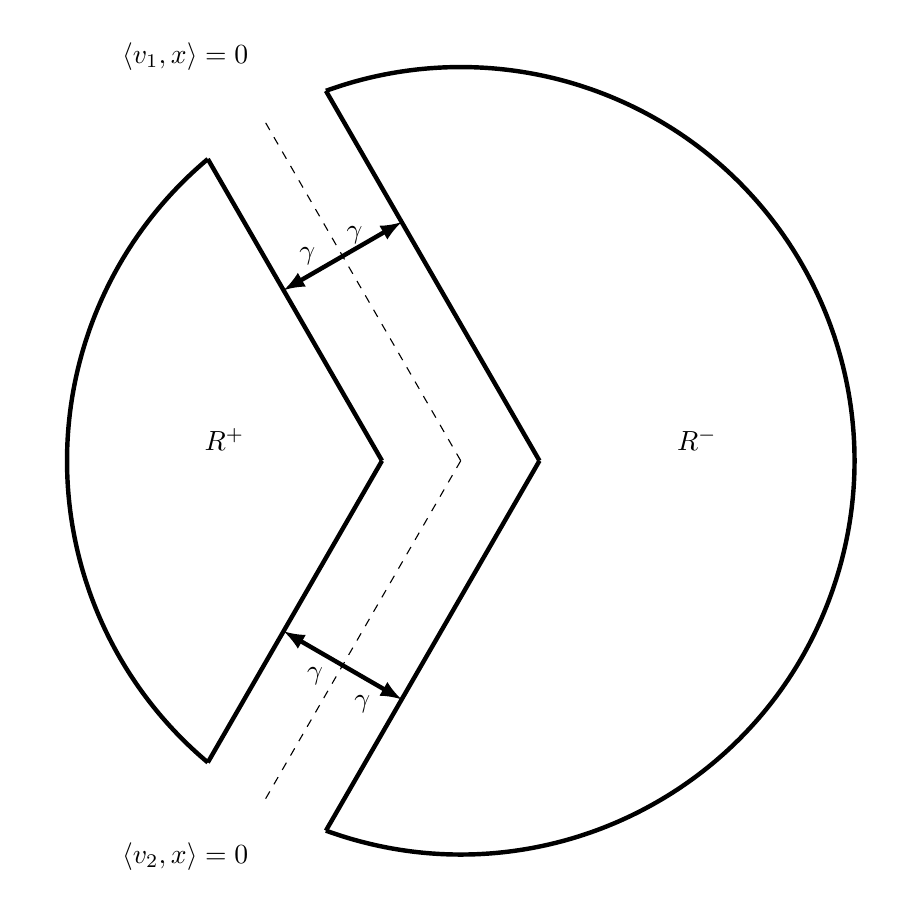
\begin{tikzpicture}

  \useasboundingbox (-5.5,-5.5) rectangle (5.5,5.5);
  % \draw[help lines] (-5.5,-5.5) rectangle (5.5,5.5);

  % Grid and coordinate axes
  %% \draw[help lines] (-5.2,-5.2) grid (5.2,5.2);
  %% \draw[thick, ->, >=latex] (-5.2,0) -- (5.2,0);
  %% \draw[thick, ->,  >=latex] (0,-5.2) -- (0,5.2);

  % Notable points
  \coordinate (Origin) at (0,0);

  \coordinate [label={[xshift=-10mm, yshift=5mm]$\ip{v_1}{x} = 0$}] (A) at (120:5);
  \coordinate [label={[xshift=-10mm, yshift=-10mm]$\ip{v_2}{x} = 0$}] (B) at (240:5);

  % Circle which contains all the examples.
  % \draw (Origin) circle (5cm);

  \draw[dashed] (Origin) -- (A);
  \draw[dashed] (Origin) -- (B);

  \coordinate (A1) at ($(120:0.5*sqrt{97} - 0.5) - (1,0)$);
  \coordinate (B1) at ($(240:0.5*sqrt{97} - 0.5) - (1,0)$);

  \coordinate (A2) at ($(120:0.5*sqrt{97} + 0.5) + (1,0)$);
  \coordinate (B2) at ($(240:0.5*sqrt{97} + 0.5) + (1,0)$);

  \draw[ultra thick] ($(Origin) - (1,0)$) -- (A1);
  \draw[ultra thick] ($(Origin) - (1,0)$) -- (B1);

  \draw[ultra thick] ($(Origin) + (1,0)$) -- (A2);
  \draw[ultra thick] ($(Origin) + (1,0)$) -- (B2);

  \pic [ultra thick, draw, angle radius=5cm] {angle=A1--Origin--B1};
  \pic [ultra thick, draw, angle radius=5cm] {angle=B2--Origin--A2};


  \coordinate (C) at (120:3);
  \coordinate [label={[xshift=-6mm, yshift=-4mm]$\gamma$}] (C1) at ($(120:3) + (0.75, 0.43301270189221932338)$);
  \coordinate [label={[xshift=+3mm, yshift=+2mm]$\gamma$}] (C2) at ($(120:3) - (0.75, 0.43301270189221932338)$);
  \draw[<->, >=latex, ultra thick] (C1) -- (C) -- (C2);

  \coordinate (D) at (240:3);
  \coordinate [label={[xshift=+4mm, yshift=-8mm]$\gamma$}] (D1) at ($(240:3) + (-0.75, 0.43301270189221932338)$);
  \coordinate [label={[xshift=-5mm, yshift=-3mm]$\gamma$}] (D2) at ($(240:3) - (-0.75, 0.43301270189221932338)$);
  \draw[<->, >=latex, ultra thick] (D1) -- (D) -- (D2);

  \coordinate [label={$R^+$}](R1) at ($(Origin) - (3,0)$);
  \coordinate [label={$R^-$}](R2) at ($(Origin) + (3,0)$);

\end{tikzpicture}
}
\end{center}
\caption[]{The figure shows the two regions $R^+$ and $R^-$ used in parts 1 and
2 of
Theorems~\ref{theorem:polynomial-approximation-1}~and~\ref{theorem:polynomial-approximation-2}
for the case $m=d=2$ and a particular choice of vectors $v_1, v_2$ and margin
parameter $\gamma$. The separating hyperplanes $\ip{v_1}{x} = 0$ and
$\ip{v_2}{x} = 0$ are shown as dashed lines.}
\label{figure:pizza-slice}
\end{figure}

The following lemma establishes a correspondence between any multivariate
polynomial in $\R^d$ and an element in $\ell_2$, and gives an upper bound on its
norm. Its proof follows from simple algebra, which we defer to
Appendix~\ref{section:proof-norm-bound}.

\begin{lemma}[Norm bound]
\label{lemma:norm-bound}
Let $p:\R^d \to \R$ be a multivariate polynomial.
There exists $c \in \ell_2$ such that $p(x) = \ip{c}{\phi(x)}_{\ell_2}$
and $\norm{c}_{\ell_2} \le 2^{\deg(p)/2} \norm{p}$.
\end{lemma}

Using the lemma and the polynomial approximation theorems, we can prove that the
mapping $\phi$ maps any set of weakly linearly separable examples to a strongly
linearly separable set of examples. Due to space constraints, we defer the full
proof of Theorem~\ref{theorem:margin-transformation} to
Appendix~\ref{section:proof-of-theorem-margin-transformation}.

%\begin{proof}[Proof sketch of Theorem~\ref{theorem:margin-transformation}]
%Since the examples $(x_1, y_1)$,  $\dots$, $(x_T, y_T)$ are weakly
%linearly separable with margin $\gamma$, there are vectors $w_1, w_2, \dots, w_K$
%satisfying \eqref{equation:weak-linear-separability-1} and
%\eqref{equation:weak-linear-separability-2}.

%Fix any $i \in \{1,2,\dots,K\}$. Consider the $K-1$ vectors $(w_i - w_j)/2$ for
%$j \in \{1,2,\dots,K\} \setminus \{i\}$. Note that the vectors have norm at most
%$1$. We consider two cases regarding the relationship between $\gamma_1$ and
%$\gamma_2$.

%\paragraph{Case 1: $\gamma_1 \geq \gamma_2$.} In this setting,
%Theorem~\ref{theorem:polynomial-approximation-1} implies that there exist a
%multivariate polynomial $p_i:\R^d \to \R$

%\begin{align*}
%\deg(p_i) & = \lceil \log_2(2K-2) \rceil \cdot \left\lceil \sqrt{{2}/{\gamma}} \right\rceil \; ,
%\end{align*}
%such that all examples $x$ in $R_i^+$ (resp. $R_i^-$) satisfy $p_i(x) \geq 1/2$
%(resp. $p_i(x) \leq -1/2$).
%Therefore, for all $t=1,2,\dots,T$, if $y_t = i$ then $p_i(x_t) \ge 1/2$,
% and if $y_t \neq i$ then $p_i(x_t) \le -1/2$, and
%\begin{align*}
%&\norm{p_i}
%\\
%& \le
%\left[
%  188 \lceil \log_2(2K-2) \rceil \cdot \left \lceil \sqrt{{2}/{\gamma}} \right \rceil
%\right]^{
%  \frac{\lceil \log_2(2K-2) \rceil \cdot \left \lceil \sqrt{{2}/{\gamma}} \right \rceil }{2}
%} \; . \\
%\end{align*}
%By \autoref{lemma:norm-bound}, there exists $c_i \in \ell_2$ such that
%$\ip{c_i}{\phi(x)}_{\ell_2} = p_i(x)$, and
%\begin{align*}
%&\norm{c_i}_{\ell_2}
%\\
%& \le
%\left[
%  376 \lceil \log_2(2K-2) \rceil \cdot \left \lceil \sqrt{{2}/{\gamma}} \right \rceil
%\right]^{
%  \frac{\lceil \log_2(2K-2) \rceil \cdot \left \lceil \sqrt{{2}/{\gamma}} \right \rceil}{2}
%} \; .
%\end{align*}
%Define vectors $u_i \in \ell_2$ as
%\begin{align*}
%u_i & =
%\frac{c_i/\sqrt{K}}{
%  \left[
%    376 \lceil \log_2(2K-2) \rceil \cdot \left \lceil \sqrt{{2}/{\gamma}} \right \rceil
%  \right]^{
%    \frac{\lceil \log_2(2K-2) \rceil \cdot \left \lceil \sqrt{\frac{2}{\gamma}} \right \rceil}{2}
%  }
%} \; . \\
%\end{align*}

%Then, $\norm{u_1}^2 + \norm{u_2}^2 + \dots + \norm{u_K}^2 \le 1$.
%Futhermore, for all $t=1,2,\dots,T$, $\ip{u_{y_t}}{x_t} \ge \gamma_1$
%and for all $j \in \{1,2,\dots,K\} \setminus \{y_t\}$,
%$\ip{u_j}{x_t} \le - \gamma_1$. In other words,
%$(\phi(x_1), y_1), (\phi(x_2), y_2), \dots, (\phi(x_T), y_T)$ are
%strongly linearly separable with margin $\gamma_1 = \max\{\gamma_1, \gamma_2\}$.

%\paragraph{Case 2: $\gamma_1 \leq \gamma_2$.} Following the
%same idea as Case 1 and using Theorem~\ref{theorem:polynomial-approximation-1},
%we can show that
%$(\phi(x_1), y_1), (\phi(x_2), y_2), \dots, (\phi(x_T), y_T)$ are
%strongly linearly separable with margin $\gamma_2 = \max\{\gamma_1, \gamma_2\}$.

%In summary, the examples are strongly
%linearly separable with margin $\gamma' = \max\{\gamma_1, \gamma_2\}$.
%Finally, observe that for any $t=1,2,\dots,T$,
%\[
%k(x_t,x_t) = \frac{1}{1 - \frac{1}{2} \norm{x_t}^2} \le 2 \; .
%\qedhere
%\]
%\end{proof}

 \section{Experiments}
\label{sec:experiments}
\begin{figure}
    \centering
    \begin{subfigure}[b]{0.23\textwidth} 
        \captionsetup{justification=centering}
        \begin{center}
        \hspace*{-0.3cm} 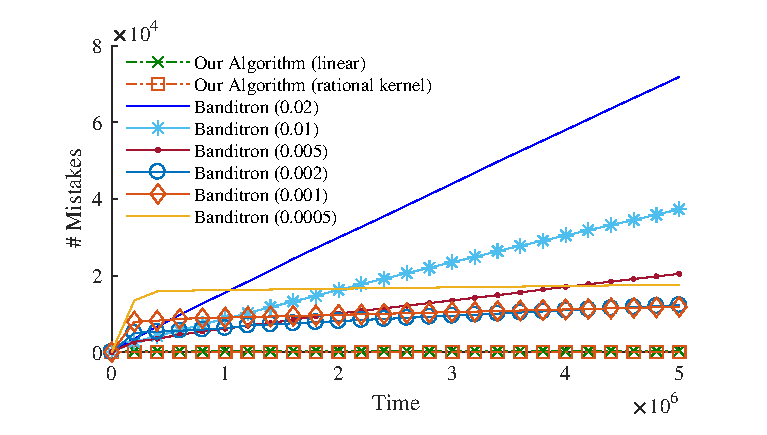
\includegraphics[width=1.15\textwidth, trim={0, 0.1cm, 0, 0}, clip]{figures/strong3}
        \caption{Strongly separable case}
        \end{center}
    \end{subfigure}
    \hfill
    \begin{subfigure}[b]{0.23\textwidth} 
        \captionsetup{justification=centering}
        \centering
        \hspace*{-0.3cm}  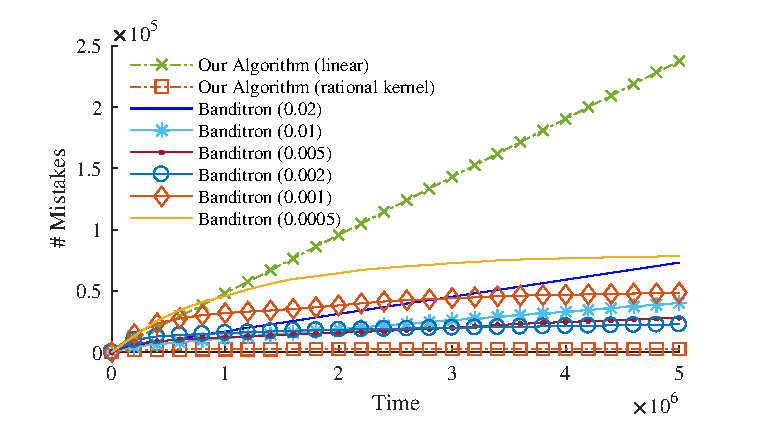
\includegraphics[width=1.15\textwidth, trim={0, 0.1cm, 0, 0}, clip]{figures/weak3}
        \caption{Weakly separable case}
    \end{subfigure}
    \vspace*{-0.2cm}
    \caption{Comparison between our algorithm and Banditron with different exploration parameter $\epsilon$ under $\gamma=0.05$ and $K=3$. }
    %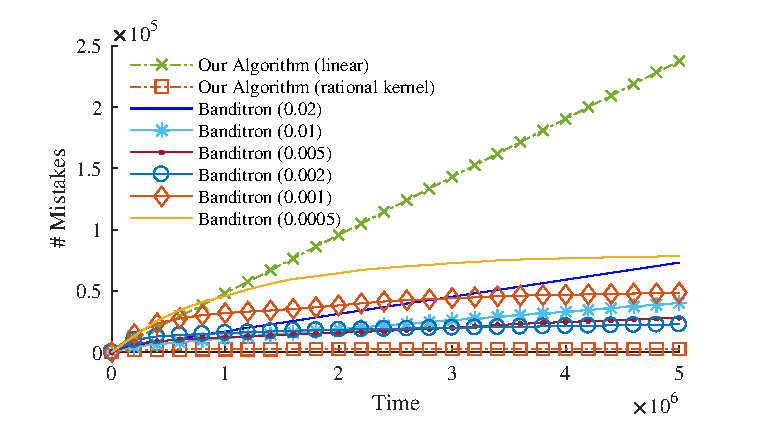
\includegraphics[width=0.25\textwidth]{figures/weak3}
    \label{fig:both}
\end{figure}

We compare our algorithm with \textsc{Banditron} empirically to show that our kernelized bandit algorithm can have significant advantage over \textsc{Banditron} is the separable case. 

We generate strongly and weakly separable samples with $K=3$ in a similar sense to those in Figure~\ref{figure:weakly-linearly-separable-examples-with-margin}. They are originally generated in a $d=2$ plate, and then lifted to $d=3$ by adding a constant feature. We provide the figures of their exact look in Appendix~\ref{sec:supp-to-experiment}. Different from Figure~\ref{figure:weakly-linearly-separable-examples-with-margin}, the three classes are non-uniform and imbanlanced: class 1 occupies a smaller sector between $-15^\circ$ and $15^\circ$, while class 2 and class 3 occupy $[15^\circ, 180^\circ]$ and $[-180^\circ, -15^\circ]$ respectively. On the other hand, $80\%$ of data comes from class 1, while $10\%$ comes from class 2 and 3 each. 

In real world, data can often be non-uniform and imbalanced. We demonstrate that \textsc{Banditron} is weak especially under these situations, while our algorithm still performs well.

We choose sample size as $5\times 10^6$ and margin as $\gamma=0.05$ (in both strongly weakly separable cases). All results are averaged over $20$ runs. 

We plot the number of mistakes against time in Figure~\ref{fig:both}. We can see there is indeed a dilemma for \textsc{Banditron}: when picking a relatively large exploration rate, it suffers from the cost of continuous exploration; when picking a relatively small exploration rate, it cannot adapt its model quickly enough (this problem exacerbates when a majority class occupies a small region, like class 1). Striking a balance between the two extremes leads to the $\sqrt{T}$ mistake bound. On the contrary, our algorithm makes significant progress on every mistake it makes, leading to a finite mistake bound.  

\section*{Acknowledgments} We thank Francesco Orabona and Wen Sun
for helpful initial discussions, and thank Adam Klivans and Rocco \mbox{Servedio} for helpful
discussions on~\citep{Klivans-Servedio-2008} and
pointing out the reference~\citep{Klivans-Servedio-2004}. We also thank Dylan Foster, 
Akshay \mbox{Krishnamurthy}, and Haipeng Luo for providing a candidate solution to our problem. 
Finally, we thank Shang-En Huang and \mbox{Mengxiao} Zhang for helpful discussions on the hardness results. 

\bibliography{biblio}
%\bibliographystyle{plainnat}
\bibliographystyle{icml2019}



% For actual submission remove everything below.
% Use appendices only in supplementray material.
\onecolumn
\appendix
\clearpage



\section{Multiclass Perceptron}
\label{section:multiclass-perceptron-proofs}

\textsc{Multiclass Perceptron} is an algorithm for \textsc{Online Multiclass
Classification}. Both the protocol for the problem and the algorithm are stated
below. The algorithm assumes that the feature vectors come from an inner product
space $(V, \ip{\cdot}{\cdot})$.

Two results are folklore. The first result is
\autoref{theorem:multiclass-perceptron-mistake-upper-bound} which states that if
examples are linearly separable with margin $\gamma$ and examples have norm
at most $R$ then the algorithm makes at most $\lfloor 2 (R/\gamma)^2 \rfloor$
mistakes. The second result is
\autoref{theorem:online-multiclass-classification-mistake-lower-bound} which
states that under the same assumptions as in
\autoref{theorem:online-multiclass-classification-mistake-lower-bound}
\emph{any} deterministic algorithm for \textsc{Online Multiclass Classification}
must make at least $\lfloor (R/\gamma)^2 \rfloor$ mistakes in the worst case.

\begin{protocol}[h]
\caption{\textsc{Online Multiclass Classification}
\label{algorithm:mutliclass-classification}}
\textbf{Require:} Number of classes $K$, number of rounds $T$. \\
\textbf{Require:} Inner product space $(V,\ip{\cdot}{\cdot})$. \\
\For{$t=1,2,\dots,T$}{
Adversary chooses example $(x_t, y_t) \in V \times \{1,2,\dots,K\}$, where $x_t$ is revealed to the learner.\\
Predict class label $\widehat y_t \in \{1,2,\dots,K\}$.\\
Observe feedback $y_t$
}
\end{protocol}

\begin{algorithm}[h]
\caption{\textsc{Multiclass Perceptron}
\label{algorithm:mutliclass-perceptron}}
\textbf{Require:} Number of classes $K$, number of rounds $T$. \\
\textbf{Require:} Inner product space $(V,\ip{\cdot}{\cdot})$. \\
Initialize $w_1^{(1)} = w_2^{(1)} = \dots = w_K^{(1)} = 0$ \\
\For{$t=1,2,\dots,T$}{
  Observe feature vector $x_t \in V$ \\
  Predict $\widehat y_t = \argmax_{i \in \{1,2,\dots,K\}} \ip{w_t^{(i)}}{x_t}$ \\
  Observe $y_t \in \{1,2,\dots,K\}$ \\
  \If{$\widehat y_t \neq y_t$}{
    Set $w_i^{(t+1)} = w_i^{(t)}$ \\ \qquad for all $i \in \{1,2,\dots,K\} \setminus \{y_t, \widehat y_t\}$ \\
    Update $w_{y_t}^{(t+1)} = w_{y_t}^{(t)} + x_t$ \\
    Update $w_{\widehat y_t}^{(t+1)} = w_{\widehat y_t}^{(t)} - x_t$ \\
  }
  \Else{
    Set $w_i^{(t+1)} = w_i^{(t)}$ for all $i \in \{1,2,\dots,K\}$ \\
  }
}
\end{algorithm}

\begin{theorem}[Mistake upper bound~\cite{Crammer-Singer-2003}]
\label{theorem:multiclass-perceptron-mistake-upper-bound}
Let $(V, \ip{\cdot}{\cdot})$ be an inner product space, let $K$ be a positive
integer, let $\gamma$ be a positive real number and let $R$ be a non-negative real
number. If $(x_1, y_1), (x_2, y_2), \dots, (x_T, y_T)$ is a sequence of labeled
examples in $V \times \{1,2,\dots,K\}$ that are weakly linearly separable with margin
$\gamma$ and $\norm{x_1}, \norm{x_2}, \dots, \norm{x_T} \le R$
then \textsc{Multiclass Perceptron} algorithm makes at most $\lfloor
2(R/\gamma)^2 \rfloor$ mistakes.
\end{theorem}

\begin{proof}
Let $M = \sum_{t=1}^T \indicator{\widehat y_t \neq y_t}$ be the number of
mistakes the algorithm makes. Since the $K$-tuple $(w_1^{(t)}, w_2^{(t)}, \dots,
w_K^{(t)})$ changes only if a mistake is made, we can upper bound $\sum_{i=1}^K
\norm{w_i^{(t)}}^2$ in terms of number of mistakes.
If a mistake happens in round $t$ then
\begin{align*}
& \sum_{i=1}^K \norm{w_i^{(t+1)}}^2 \\
& = \left(\sum_{i \in \{1,2,\dots,K\} \setminus \{y_t, \widehat y_t\} } \norm{w_i^{(t)}}^2 \right) \\
& \qquad + \norm{w_{y_t}^{(t)} + x_t}^2 + \norm{w_{\widehat y_t}^{(t)} - x_t}^2 \\
& = \left(\sum_{i \in \{1,2,\dots,K\} \setminus \{y_t, \widehat y_t\} } \norm{w_i^{(t)}}^2 \right) + \norm{w_{y_t}^{(t)}}^2 + \norm{w_{\widehat y_t}^{(t)}}^2 \\
& \qquad + 2 \norm{x_t}^2 + 2 \ip{w_{y_t}^{(t)} - w_{\widehat y_t}^{(t)}}{x_t} \\
& = \left(\sum_{i=1}^K \norm{w_i^{(t)}}^2 \right) + 2 \norm{x_t}^2 + 2 \ip{w_{y_t}^{(t)} - w_{\widehat y_t}^{(t)}}{x_t} \\
& \le \left(\sum_{i=1}^K \norm{w_i^{(t)}}^2 \right) + 2 \norm{x_t}^2 \\
& \le \left(\sum_{i=1}^K \norm{w_i^{(t)}}^2 \right) + 2 R^2 \; .
\end{align*}
So each time a mistake happens, $\sum_{i=1}^K \norm{w_i^{(t)}}^2$ increases by at most $2R^2$. Thus,
$$
\sum_{i=1}^K \norm{w_i^{(T+1)}}^2 \le 2R^2 M \; .
$$
Let $w_1^*, w_2^*, \dots, w_K^* \in V$ be vectors satisfying the
\eqref{equation:weak-linear-separability-1} and
\eqref{equation:weak-linear-separability-2}. We lower bound $\sum_{i=1}^K \ip{w_i^*}{w_i^{(t)}}$. This quantity changes
only when a mistakes happens. If mistake happens in round $t$, we have
\begingroup
\allowdisplaybreaks
\begin{align*}
& \sum_{i=1}^K \ip{w_i^*}{w_i^{(t+1)}} \\
& = \left( \sum_{i \in \{1,2,\dots,K\} \setminus \{y_t, \widehat y_t\}} \ip{w_i^*}{w_i^{(t)}} \right) \\
& \qquad + \ip{w_{y_t}^*}{w_{y_t}^{(t)} + x_t} + \ip{w_{\widehat y_t}^*}{w_{\widehat y_t}^{(t)} - x_t} \\
& = \left( \sum_{i=1}^K \ip{w_i^*}{w_i^{(t)}} \right) + \ip{w_{y_t}^* - w_{\widehat y_t}^*}{x_t} \\
& \ge  \left( \sum_{i=1}^K \ip{w_i^*}{w_i^{(t)}} \right) + \gamma \; .
\end{align*}
\endgroup
Thus, after $M$ mistakes,
$$
\sum_{i=1}^K \ip{w_i^*}{w_i^{(T+1)}} \ge \gamma M \; .
$$
We upper bound the left hand side by using Cauchy-Schwartz inequality twice and
the condition \eqref{equation:weak-linear-separability-1} on $w_1^*, w_2^*, \dots,
w_K^*$. We have
\begin{align*}
\sum_{i=1}^K \ip{w_i^*}{w_i^{(T+1)}}
& \le \sum_{i=1}^K \norm{w_i^*} \cdot \norm{w_i^{(T+1)}} \\
& \le \sqrt{\sum_{i=1}^K \norm{w_i^*}^2} \sqrt{\sum_{i=1}^K \norm{w_i^{(T+1)}}^2} \\
& \le \sqrt{\sum_{i=1}^K \norm{w_i^{(T+1)}}^2} \; .
\end{align*}
Combining all inequalities, we get
$$
(\gamma M)^2 \le \sum_{i=1}^K \norm{w_i^{(T+1)}}^2 \le 2R^2 M \; .
$$
We conclude that $M \le 2(R/\gamma)^2$. Since $M$ is an integer, $M \le \lfloor 2(R/\gamma)^2 \rfloor$.
\end{proof}


\begin{theorem}[Mistake lower bound]
\label{theorem:online-multiclass-classification-mistake-lower-bound}
Let $K$ be a positive integer, let $\gamma$ be a positive real number and let
$R$ be a non-negative real number. For any (possibly randomized) algorithm
$\calA$ for the \textsc{Online Multiclass Classification} problem there exists
an inner product space $(V, \ip{\cdot}{\cdot})$, a non-negative integer $T$ and
a sequence of labeled examples $(x_1, y_1), (x_2, y_2), \dots, (x_T, y_T)$
examples in $V \times \{1,2,\dots,K\}$ that are weakly linearly separable with
margin $\gamma$, the norms satisfy $\norm{x_1}, \norm{x_2}, \dots, \norm{x_T}
\le R$ and the algorithm makes at least $\frac 1 2 \lfloor (R/\gamma)^2 \rfloor$
mistakes.
\end{theorem}

\begin{proof}
Let $T = \lfloor (R/\gamma)^2 \rfloor$, $V = \R^T$, and for all $t$ in
$\cbr{1,\ldots,T}$, define instance $x_t = R e_t$ where $e_t$ is $t$-th element
of the standard orthonormal basis of $\R^T$.
Let labels $y_1, \ldots, y_T$ be chosen i.i.d uniformly at random from
$\cbr{1,2,\ldots,K}$ and independently of any randomness used by the algorithm
$\calA$.


%let $x_1, x_2, \dots, x_T$ be the
%orthogonal vectors such that $\norm{x_t} = R$ for all $t=1,2,\dots,T$. For
%example, we can take

%Since the algorithm is deterministic, we can construct the sequence of labels
%$y_1, y_2, \dots, y_T$ adaptively based on the predictions $\widehat y_1,
%\widehat y_2, \dots, \widehat y_T$ of the algorithm. We define $y_t$ to be any
%element of $\{1,2,\dots,K\}$ not equal to $\widehat y_t$. This way the algorithm
%makes a mistake in every round $t=1,2,\dots,T$.

We first show that the set of examples $(x_1,y_1)$, $\ldots$,
$(x_T, y_T)$ we have constructed is weakly linearly separable
with margin $\gamma$. To prove that, we demonstrate vectors $w_1, w_2, \dots, w_K$
satisfying conditions \eqref{equation:weak-linear-separability-1} and
\eqref{equation:weak-linear-separability-2}. We define
$$
w_i = \frac{\gamma}{R} \sum_{\substack{t : 1 \le t \le T \\ y_t = i}} e_t \qquad \text{for $i=1,2,\dots,K$.}
$$
Let $a_i = |\{ t ~:~ 1 \le t \le T, \ y_t = i \}|$ be the number of occurrences of label $i$.
It is easy to see that
$$
\norm{w_i}^2 = \frac{\gamma^2}{R^2} \sum_{\substack{t : 1 \le t \le T \\ y_t = i}} \norm{e_t}^2 = \frac{a_i \gamma^2}{R^2} \qquad \text{for $i=1,2,\dots,K$.}
$$
Since $\sum_{i=1}^K a_i = T$,
$\sum_{i=1}^K \norm{w_i}^2 = T \cdot \frac{\gamma^2}{R^2} \leq 1$, i.e.
the condition
\eqref{equation:weak-linear-separability-1} holds. To verify condition
\eqref{equation:weak-linear-separability-2} consider any labeled example $(x_t,
y_t)$. Then, for any $i$ in $\cbr{1,\ldots,K}$, by the definition of $w_i$, we have
\begin{align*}
\ip{w_i}{x_t}
& = \frac{\gamma}{R} \sum_{\substack{s : 1 \le s \le T \\ y_s = i}} \ip{e_s}{R e_t} \\
& = \gamma \cdot \sum_{\substack{s : 1 \le s \le T \\ y_s = i}} \indicator{s = t} \\
& = \gamma \cdot \indicator{y_t = i}
\; .
\end{align*}
Therefore, if $i = y_t$, $\ip{w_i}{x_t} = \gamma$;
otherwise $i \neq y_t$, in which case $\ip{w_i}{x_t} = 0$.
Hence, condition \eqref{equation:weak-linear-separability-2} holds.

We now give a lower bound on the number of mistakes $\calA$ makes.
As $y_t$ is chosen uniformly from $\{1,2,\dots,K\}$ and independent of
$\calA$'s randomization
$$
\Exp[ \indicator{\widehat y_t \neq y_t} ] \ge 1 - \frac{1}{K} \ge \frac{1}{2} \; .
$$
Summing over all $t$ in $\cbr{1,\ldots,T}$, we conclude that
$$
\Exp \sbr{ \sum_{t=1}^T \indicator{\widehat y_t \neq y_t} } \geq \frac T 2 = \frac 1 2 \lfloor (R/\gamma)^2 \rfloor,
$$
which completes the proof.
\end{proof}

%& = \frac{R}{\sqrt{T}} \\
%& \ge \frac{R}{R/\gamma} \\
%& = \gamma \; .
%and similarly, for any $i \in \{1,2,\dots,K\} \setminus \{y_t\}$ we have
%$\ip{w_i}{x_t} = 0$.

\section{Proofs of Theorems~\ref{theorem:strongly-separable-examples-mistake-upper-bound} and \ref{theorem:strongly-separable-examples-mistake-lower-bound}}
\label{section:proofs-for-stringly-separable-examples}

%$\norm{x_1}, \norm{x_2}, \dots, \norm{x_T} \le R$
%$A
%= \sum_{t ~:~ S_t \neq \emptyset} z_t$
%B = \sum_{t ~:~ S_t = \emptyset} z_t
%\sum_{t ~:~ S_t = \emptyset}
\begin{proof}[Proof of \autoref{theorem:strongly-separable-examples-mistake-upper-bound}]
Let $M = \sum_{t=1}^T z_t$ be the number of
mistakes Algorithm~\ref{algorithm:algorithm-for-strongly-linearly-separable-examples} makes.
Let $A = \sum_{t=1}^T \one[S_t \neq \emptyset] z_t$ be the number of mistakes in the rounds
when $S_t \neq \emptyset$, i.e. the number of rounds line~\ref{line:neg-update} is
executed.
In addition, let $B = \sum_{t=1}^T \one[S_t = \emptyset] z_t$ be the
number of mistakes in the rounds when $S_t = \emptyset$.
It can be easily seen that $M = A + B$.

Let $C = \sum_{t=1}^T \one[S_t = \emptyset](1 - z_t)$ be the number of rounds
line~\ref{line:pos-update} gets executed. Let
$U = \sum_{t=1}^T (\one[S_t \neq \emptyset] z_t + \one[S_t = \emptyset](1 - z_t))$
be the number of rounds line~\ref{line:pos-update} or~\ref{line:neg-update}
gets executed. In other words, $U$ is the number of times the $K$-tuple of
vectors $(w_1^{(t)}, w_2^{(t)}, \dots, w_K^{(t)})$ gets updated. It can be
easily seen that $U = A + C$.

The key observation is that $\Exp[B] = (K-1) \Exp[C]$.
To see this, note that if $S_t = \emptyset$, there is $1/K$ probability that the algorithm
guesses the correct label ($z_t = 0$) and with probability $(K-1)/K$ algorithm's guess is
incorrect ($z_t = 1$). Therefore,
\[ \Exp[ z_t |S_t = \emptyset] = \frac{K-1}{K}, \]
\[ \Exp[B] = \frac{K-1}{K} \Exp \sbr{ \sum_{t=1}^T \indicator{S_t = \emptyset} }, \]
\[ \Exp[C] = \frac{1}{K} \Exp \sbr{ \sum_{t=1}^T \indicator{S_t = \emptyset} }. \]

Putting all the information together, we get that
\begin{align}
\Exp[M]
& = \Exp[A] + \Exp[B] \nonumber \\
& = \Exp[A] + (K-1) \Exp[C] \nonumber \\
& \le (K-1) \Exp[A + C] \nonumber\\
& = (K-1) \Exp[U]  \; .
\label{eqn:mistake-update}
\end{align}

To finish the proof, we need to upper bound the number of updates $U$. We claim
that $U \le \lfloor 4(R/\gamma)^2 \rfloor$ with probability 1.
The proof of this upper bound is
similar to the proof of the mistake bound for \textsc{Multiclass Perceptron}
algorithm. Let $w_1^*, w_2^*, \dots, w_K^* \in V$ be vectors that satisfy
\eqref{equation:strong-linear-separability-1},
\eqref{equation:strong-linear-separability-2} and
\eqref{equation:strong-linear-separability-3}.
The $K$-tuple $(w_1^{(t)}, w_2^{(t)}, \dots, w_K^{(t)})$
changes only if there is an update in round $t$.
We investigate how $\sum_{i=1}^K \norm{w_i^{(t)}}^2$ and
$\sum_{i=1}^K \ip{w_i^*}{w_i^{(t)}}$ change. If there is an update in round $t$,
by lines~\ref{line:pos-update} and~\ref{line:neg-update}, we always have
$ w_{\widehat y_t}^{(t+1)} = w_{\widehat y_t}^{(t)} + (-1)^{z_t} x_t $,
and for all $i \neq \widehat y_t$, $w_{i}^{(t+1)} = w_{i}^{(t)}$.
Therefore,
\begingroup
\allowdisplaybreaks
\begin{align*}
& \sum_{i=1}^K \norm{w_i^{(t+1)}}^2 \\
& = \left( \sum_{i \in \{1,2,\dots,K\} \setminus \{\widehat y_t\}} \norm{w_i^{(t)}}^2 \right) + \norm{w_{\widehat y_t}^{(t+1)}}^2 \\
& = \left( \sum_{i \in \{1,2,\dots,K\} \setminus \{\widehat y_t\}} \norm{w_i^{(t)}}^2 \right) + \norm{w_{\widehat y_t}^{(t)} + (-1)^{z_t} x_t}^2 \\
& = \left( \sum_{i=1}^K \norm{w_i^{(t)}}^2 \right) + \norm{x_t}^2 + \underbrace{(-1)^{z_t} 2 \ip{w_{\widehat y_t}^{(t)}}{x_t}}_{\le 0} \\
& \le \left( \sum_{i=1}^K \norm{w_i^{(t)}}^2 \right) + \norm{x_t}^2 \\
& \le \left( \sum_{i=1}^K \norm{w_i^{(t)}}^2 \right) + R^2 \; .
\end{align*}
\endgroup
The inequality that $(-1)^{z_t} 2 \ip{w_{\widehat y_t}^{(t)}}{x_t} \leq 0$ is from a case analysis: if line~\ref{line:pos-update} is executed, then $z_t = 0$ and $\ip{w_i^{(t)}}{x_t} \ge 0$; otherwise line~\ref{line:neg-update} is executed, in which case $z_t = 1$ and $\ip{w_i^{(t)}}{x_t} \le 0$.


Hence, after $U$ updates,
\begin{equation}
\sum_{i=1}^K \norm{w_i^{(T+1)}}^2 \le R^2 U \; .
\label{eqn:norm-ub}
\end{equation}
Similarly, if there is an update in round $t$, we have
\begingroup
\allowdisplaybreaks
\begin{align*}
& \sum_{i=1}^K \ip{w_i^*}{w_i^{(t)}} \\
& = \left( \sum_{i \in \{1,2,\dots,K\} \setminus \{\widehat y_t\}} \ip{w_i^*}{w_i^{(t)}} \right) + \ip{w_{\widehat y_t}^*}{w_{\widehat y_t}^{(t+1)}} \\
& = \left( \sum_{i \in \{1,2,\dots,K\} \setminus \{\widehat y_t\}} \ip{w_i^*}{w_i^{(t)}} \right) \\
& \qquad + \ip{w_{\widehat y_t}^*}{w_{\widehat y_t}^{(t)} + (-1)^{z_t} x_t} \\
& = \left( \sum_{i=1}^K \ip{w_i^*}{w_i^{(t)}} \right) + (-1)^{z_t} \ip{w_{\widehat y_t}^*}{x_t} \\
& \ge \left( \sum_{i=1}^K \ip{w_i^*}{w_i^{(t)}} \right) + \frac \gamma 2,
\end{align*}
\endgroup
where the last inequality follows from a case analysis on $z_t$ and
Definition~\ref{definition:weak-linear-separability}: if $z_t = 0$, then
$\widehat y_t = y_t$, by Equation~\eqref{equation:strong-linear-separability-2},
we have that $\ip{w_{\widehat y_t}^*}{x_t} \geq \frac \gamma 2$; if $z_t = 1$,
then $\widehat y_t \neq y_t$, by
Equation~\eqref{equation:strong-linear-separability-3}, we have that
$\ip{w_{\widehat y_t}^*}{x_t} \le -\frac \gamma 2$.

Thus, after $U$ updates,
\begin{equation}
\sum_{i=1}^K \ip{w_i^*}{w_i^{(T+1)}} \ge \frac {\gamma U} 2 \; .
\label{eqn:norm-lb}
\end{equation}
Applying Cauchy-Schwartz's inequality twice, and using assumption
\eqref{equation:strong-linear-separability-1}, we get that
\begin{align*}
\sum_{i=1}^K \ip{w_i^*}{w_i^{(T+1)}}
& \le \sum_{i=1}^K \norm{w_i^*} \cdot \norm{w_i^{(T+1)}} \\
& \le \sqrt{\sum_{i=1}^K \norm{w_i^*}^2} \sqrt{\sum_{i=1}^K \norm{w_i^{(T+1)}}^2} \\
& \le \sqrt{\sum_{i=1}^K \norm{w_i^{(T+1)}}^2} \; .
\end{align*}
Combining the above inequality with Equations~\eqref{eqn:norm-ub} and~\eqref{eqn:norm-lb}, we get
$$
\left(\frac{\gamma U}{2} \right)^2 \le \sum_{i=1}^K \norm{w_i^{(T+1)}}^2 \le R^2 U \; .
$$
We conclude that $U \le 4(R/\gamma)^2$. Since $U$ is an integer, $U \le \lfloor 4(R/\gamma)^2 \rfloor$.

Applying Equation~\eqref{eqn:mistake-update}, we get
$$
\Exp[M] \leq (K-1) \Exp[U] \leq (K-1) \lfloor 4(R/\gamma)^2 \rfloor \; . \qedhere
$$
\end{proof}




\begin{proof}[Proof of \autoref{theorem:strongly-separable-examples-mistake-lower-bound}]
We use probabilistic method. Let $M = \left\lfloor \frac{1}{4} (R/\gamma)^2
\right\rfloor$. Let $V = \R^{M+1}$ equipped with the standard inner product.
Let $e_1, e_2, \dots, e_{M+1}$ be the standard orthonormal basis of $V$. We
define vectors $v_1, v_2, \dots, v_M \in V$ where $v_j = \frac{R}{\sqrt{2}}(e_j
+ e_{M+1})$ for $j=1,2,\dots,M$. Let $\ell_1, \ell_2, \dots, \ell_M$ be chosen
i.i.d. uniformly at random from $\{1,2,\dots,K\}$ and independently of any
randomness used the by algorithm $\calA$. Let $T = M (K - 1)$. We define examples $(x_1,
y_1), (x_2, y_2), \dots, (x_T, y_T)$ as follows. For any $j=1,2,\dots,M$ and any
$h=1,2,\dots,K-1$,
$$
(x_{(j-1)(K-1) + h}, y_{(j-1)(K-1) + h}) = (v_j, \ell_j)
$$


With probability one, the norm of each example is exactly $R$.
We show that with probability
one, the examples are strongly separable with margin $\gamma$. To see
that, consider $w_1^*, w_2^*, \dots, w_K^* \in V$ defined by
$$
w_i^* = \sqrt{2} \frac{\gamma}{R} \left( \sum_{j ~:~ \ell_j = i} e_j \right) - \frac{\sqrt{2}}2 \frac{\gamma}{R} e_{M+1}
$$
for $i=1,2,\dots,K$.

for $i \in \{1,2,\dots,K\}$ and $j \in
\{1,2,\dots,M\}$, we consider the inner product of $w_i^*$ and $v_j$.
If $i = \ell_j$, $\ip{w_i^*}{v_j} = \gamma - \frac \gamma 2 = \frac \gamma 2$;
otherwise $i \neq \ell_j$, in which case
$\ip{w_i^*}{v_j} = 0 - \frac \gamma 2 = - \frac \gamma 2$.
This means that $w_1^*, w_2^*, \dots, w_K^*$ satisfy
conditions
\eqref{equation:strong-linear-separability-2} and
\eqref{equation:strong-linear-separability-3}. Condition \eqref{equation:strong-linear-separability-1}
is satisfied since
\begin{multline*}
\sum_{i=1}^K \norm{w_i^*}^2
= 2 \frac{\gamma^2}{R^2} \sum_{j=1}^M \norm{e_j}^2 +  \frac{\gamma^2}{2 R^2} K \norm{e_{M+1}}^2 \\
= 2 \frac{\gamma^2}{R^2} M + \frac{\gamma^2}{2 R^2} K
\le \frac{1}{2} + \frac{1}{2}
= 1 \; .
\end{multline*}

It remains to lower bound the expected number of mistakes of $\calA$. For
any $j \in \{1,2,\dots,M\}$, consider the expected number of mistakes the
algorithm makes in rounds $(K-1)(j-1) + 1, (K-1)(j-1) + 2, \dots, (K-1)j$.

Define a filtration $\cbr{\calB_j}_{j=0}^M$,
where $\calB_j = \sigma((x_1, y_1, \hat{y}_1), \ldots, (x_{(K-1)j}, y_{(K-1)j}, \hat{y}_{(K-1)j}))$
for every $j$ in $\{1,2,\dots,M\}$.
By Claim 2 of~\citet{Daniely-Helbertal-2013}, as $\ell_j$
is chosen uniformly from $\cbr{1,\dots,K}$ and independent of $\calB_{j-1}$ and $\calA$'s
randomness,
$$
\Exp \sbr{ \sum_{t=(K-1)(j-1) + 1}^{(K-1)j} z_t ~\Bigg|~ \calB_{j-1} } \geq \frac{K-1}2 \; .
$$
This implies that
$$
\Exp \sbr{ \sum_{t=(K-1)(j-1) + 1}^{(K-1)j} z_t } \ge \frac{K-1}2 \; .
$$
Summing over all $j$ in $\{1,2,\dots,M\}$,
$$
\Exp \sbr{ \sum_{t=1}^{(K-1)M} z_t} \geq \frac{K-1}2 \cdot M = \frac{K-1}2 \left\lfloor \frac 1 4 (R/\gamma)^2 \right\rfloor \; .
$$

%In these rounds,
%the algorithm is guessing the label $\ell_j$. Since $\ell_j$ is chosen uniformly
%at random from the set $\{1,2,\dots,K\}$ and feedback is only binary, the
%expected number of mistakes the algorithm makes in these rounds is at least
%$\frac{K-1}{2}$. Altogether, the algorithm makes at least $\frac{K-1}{2} M$
%mistakes in expectation.

%\chicheng{I think this part need to be formalized, by directly using
%~\cite{Daniely-Helbertal-2013}, Claim 2.}
%Can we assume without loss of generality
%that a deterministic prediction algorithm will have a smaller expected cost?
%If so, define $F(k)$ be the number of mistake that will be made by the algorithm,
%if the adversary commits to a label uniformly at random from $\cbr{1,2,\ldots,k}$,
%and the guessing of the label lasts for $k$ rounds.
%we can construct a recurrence of $F$: $F(k) = F(k-1) + \frac{k-1}{k}$, and $F(1) = 0$.
%Therefore, $F(K) = \Omega(K)$.

Finally, since strong separability and norm condition hold with probability one,
there exists a particular (i.e. deterministic) sequence of examples for which
the algorithm makes at least $\frac{K-1}2 \left\lfloor \frac 1 4 (R/\gamma)^2
\right\rfloor$ mistakes in expectation over its internal randomization.
\end{proof}

\section{Proof of Lemma~\ref{lemma:norm-bound}}
\label{section:proof-norm-bound}

\begin{proof}
Note that the polynomial $p$ can be written as
$p(x) = \sum_{\alpha_1, \alpha_2, \dots, \alpha_d} c'_{\alpha_1, \alpha_2, \dots, \alpha_d} x_1^{\alpha_1} x_2^{\alpha_2} \dots x_d^{\alpha_d}$.
We define $c \in \ell_2$ using the multi-index notation as
$$
c_{\alpha_1, \alpha_2, \dots, \alpha_d}
= \frac{c'_{\alpha_1, \alpha_2, \dots, \alpha_d} 2^{(\alpha_1 + \alpha_2 + \dots + \alpha_d)/2}}{\sqrt{\binom{\alpha_1 + \alpha_2 + \dots + \alpha_d}{\alpha_1, \alpha_2, \dots, \alpha_d}}}
$$
for all tuples $(\alpha_1, \alpha_2, \dots, \alpha_d)$ such that $\alpha_1 + \alpha_2 + \dots + \alpha_d \le \deg(p)$.
Otherwise, we define $c_{\alpha_1, \alpha_2, \dots, \alpha_d} = 0$. By the definition
of $\phi$, $\ip{c}{\phi(x)}_{\ell_2} = p(x)$.

Whether $\alpha_1 + \ldots + \alpha_d \leq \deg(p)$, we always have:
\begin{align*}
|c_{\alpha_1, \alpha_2, \dots, \alpha_d}|
 \le 2^{(\alpha_1 + \alpha_2 + \dots + \alpha_d)/2} |c'_{\alpha_1, \alpha_2, \dots, \alpha_d}|
 \le 2^{\deg(p)/2} |c'_{\alpha_1, \alpha_2, \dots, \alpha_d}| \; .
\end{align*}
Therefore,
\begin{align*}
\norm{c}_{\ell_2}
 \le 2^{\deg(p)/2} \sqrt{\sum_{\alpha_1, \alpha_2, \dots, \alpha_d} (c'_{\alpha_1, \alpha_2, \dots, \alpha_d})^2} 
 = 2^{\deg(p)/2} \norm{p} \; . \qquad \qedhere
\end{align*}
\end{proof}

\section{Proof of Theorems~\ref{theorem:polynomial-approximation-1}~and~\ref{theorem:polynomial-approximation-2}}
\label{section:proof-of-polynomial-approximation}

In this section, we follow the construction of~\citet{Klivans-Servedio-2008}
(which in turn uses the constructions of~\citet{Beigel-Reingold-Spielman-1995})
to establish two polynomials of low norm, such that it takes large positive values
in
\[ \bigcap_{i=1}^m \left\{ x \in \R^d ~:~ \norm{x} \le 1, \ \ip{v_i}{x} \ge \gamma \right\} \]
and takes large negative values in
\[ \bigcup_{i=1}^m \left\{ x \in \R^d ~:~ \norm{x} \le 1, \ \ip{v_i}{x} \le -\gamma \right\} . \]
We improve the norm bound analysis of~\citet{Klivans-Servedio-2008} in two aspects:
\begin{enumerate}
  \item Our upper bounds on the norm of the polynomials do not have any dependency on the
  dimensionality $d$.
  \item We remove the requirement that the fractional part of input $x$ must be above some threshold in
  Theorem~\ref{theorem:polynomial-approximation-2}.
\end{enumerate}
A lot of the proof details are similar to those of~\citet{Klivans-Servedio-2008}; nevertheless,
we provide a self-contained full proof here.

For the proofs of the theorems we need several auxiliary results.

\begin{lemma}[Simple inequality]
\label{lemma:simple-inequality}
For any real numbers $b_1, b_2, \dots, b_n$,
$$
\left( \sum_{i=1}^n b_i \right)^2 \le n \sum_{i=1}^n b_i^2 \; .
$$
\end{lemma}

\begin{proof}
The lemma follows from Cauchy-Schwartz inequality applied to
vectors $(b_1, b_2, \dots, b_n)$ and $(1,1,\dots,1)$.
\end{proof}

\begin{lemma}[Bound on binomial coefficients]
\label{lemma:binomial-bound}
For any integers $n,k$ such that $n \ge k \ge 0$,
$$
\binom{n}{k} \le (n - k + 1)^k \; .
$$
\end{lemma}

\begin{proof}
If $k = 0$, the inequality trivially holds. For the rest of the proof we can
assume $k \ge 1$. We write the binomial coefficient as
\begin{align*}
\binom{n}{k}
& = \frac{n(n-1)\cdots(n-k+1)}{k(k-1) \cdots 1} \\
& = \frac{n}{k} \cdot \frac{n-1}{k - 1} \cdots \frac{n-k+1}{1} \; .
\end{align*}
We claim that
$$
\frac{n}{k} \le \frac{n-1}{k - 1} \le \cdots \le \frac{n-k+1}{1}
$$
from which the lemma follows by upper bounding all the fractions by $n-k+1$.
It remains to prove that for any $j=0,1,\dots,k-1$,
$$
\frac{n - j + 1}{k - j + 1} \le \frac{n - j}{k - j} \; .
$$
Multiplying by the (positive) denominators, we get an equivalent inequality
$$
(n - j + 1)(k - j) \le (n - j)(k - j + 1) \; .
$$
Cancelling common terms leads to an equivalent inequality
$$
k - j \le n - j \; ,
$$
which since $n \ge k$ by assumption.
\end{proof}

\begin{lemma}[Properties of the norm of polynomials]
\label{lemma:properties-of-norm-of-polynomials}
\hspace{1cm} % Dummy space
\begin{enumerate}
\item Let $p_1, p_2, \dots, p_n$ be multivariate polynomials and let $p(x) =
\prod_{j=1}^n p_j(x)$ be their product.  Then, $\norm{p}^2 \le n^{\sum_{j=1}^n
\deg(p_j)} \prod_{j=1}^n \norm{p_j}^2$.

\item Let $q$ be a multivariate polynomial of degree at most $s$ and let $p(x) =
(q(x))^n$. Then, $\norm{p}^2 \le n^{ns} \norm{q}^{2n}$.

\item Let be $p_1, p_2, \dots, p_n$ be multivariate polynomials. Then,
$\norm{\sum_{j=1}^n p_j}^2 \le n \sum_{j=1}^n \norm{p_j}^2$.
\end{enumerate}
\end{lemma}

\begin{proof}
Using multi-index notation we can write any multivariate polynomial $p$ as
$$
p(x) = \sum_A c_A x^A
$$
where $A = (\alpha_1, \alpha_2, \dots, \alpha_d)$ is a multi-index (i.e. a $d$-tuple of
non-negative integers), $x^A = x_1^{\alpha_1} x_2^{\alpha_2} \dots x_d^{\alpha_d}$ is a
monomial and $c_A = c_{\alpha_1, \alpha_2, \dots, \alpha_d}$ is the corresponding real
coefficient. The sum is over a finite subset of $d$-tuples of non-negative
integers. Using this notation, the norm of a polynomial $p$ can be written as
$$
\norm{p} = \sqrt{\sum_A (c_A)^2} \; .
$$
For a multi-index $A = (\alpha_1, \alpha_2, \dots, \alpha_d)$ we define its
$1$-norm as $\norm{A}_1 = \alpha_1 + \alpha_2 + \dots + \alpha_d$.

To prove the part 1, we express $p_j$ as
$$
p_j(x) = \sum_{A_j} c^{(j)}_{A_j} x^{A_j} \; .
$$
Since $p(x) = \prod_{i=1}^n p_j(x)$, the coefficients of its expansion $p(x) =
\sum_A c_A x^A$ are
$$
c_A = \sum_{\substack{(A_1, A_2, \dots, A_n) \\ A_1 + A_2 + \dots + A_n = A}} c^{(1)}_{A_1} c^{(2)}_{A_2} \cdots c^{(n)}_{A_n} \; .
$$
Therefore,
\begin{align*}
\norm{p}^2
& = \sum_{A} (c_A)^2 \\
& = \sum_{A} \left( \sum_{\substack{(A_1, A_2, \dots, A_n) \\ A_1 + A_2 + \dots + A_n = A}} c^{(1)}_{A_1} c^{(2)}_{A_2} \cdots c^{(n)}_{A_n} \right)^2 \\
& = \sum_{A} \left( \sum_{\substack{(A_1, A_2, \dots, A_n) \\ A_1 + A_2 + \dots + A_n = A}} \prod_{j=1}^n c^{(j)}_{A_j} \right)^2
\end{align*}
and
\begin{align*}
\prod_{i=1}^n \norm{p_i}^2
& = \prod_{i=1}^n \left( \sum_{A_i} (c^{(i)}_{A_i})^2 \right) \\
& = \sum_{(A_1, A_2, \dots, A_n)} \prod_{j=1}^n (c^{(j)}_{A_j})^2 \\
& = \sum_{(A_1, A_2, \dots, A_n)} \left( \prod_{j=1}^n c^{(j)}_{A_j} \right)^2 \\
& = \sum_A \sum_{\substack{(A_1, A_2, \dots, A_n) \\ A_1 + A_2 + \dots + A_n = A}} \left( \prod_{j=1}^n c^{(j)}_{A_j} \right)^2
\end{align*}
where in both cases the outer sum is over multi-indices $A$ such that $\norm{A}_1 \le \deg(p)$.
\autoref{lemma:simple-inequality} implies that for any multi-index $A$,
\[
\left( \sum_{\substack{(A_1, A_2, \dots, A_n) \\ A_1 + A_2 + \dots + A_n = A}} \prod_{j=1}^n c^{(j)}_{A_j} \right)^2
\le M_A \sum_{\substack{(A_1, A_2, \dots, A_n) \\ A_1 + A_2 + \dots + A_n = A}} \left( \prod_{j=1}^n c^{(j)}_{A_j} \right)^2 \; .
\]
where $M_A$ is the number of $n$-tuples $(A_1, A_2, \dots, A_n)$ such that $A_1 +
A_2 + \dots + A_n = A$.

To finish the proof, it is sufficient to prove that $M_A \le n^{\deg(p)}$ for
any $A$ such that $\norm{A}_1 \le \deg(p)$. To prove this inequality, consider a
multi-index $A = (\alpha_1, \alpha_2, \dots, \alpha_d)$ and consider its $i$-th coordinate
$\alpha_i$. In order for $A_1 + A_2 + \dots + A_n = A$ to hold, the $i$-th
coordinates of $A_1, A_2, \dots, A_n$ need to sum to $\alpha_i$. There are exactly
$\binom{\alpha_i + n - 1}{\alpha_i}$ possibilities for the choice of $i$-th
coordinates of $A_1, A_2, \dots, A_n$. The total number of choices is thus
$$
M_A = \prod_{i=1}^d \binom{\alpha_i + n - 1}{\alpha_i} \; .
$$
Using \autoref{lemma:binomial-bound}, we upper bound it as
$$
M_A \le \prod_{i=1}^d n^{\alpha_i} = n^{\norm{A}_1} \le n^{\deg(p)} \; .
$$

Part 2 follows from the part 1 by setting $p_1 = p_2 = \dots p_n = q$.

To prove part 3, we use generalized triangle inequality and
\autoref{lemma:simple-inequality}. We have
\[
\norm{\sum_{j=1}^n p_j}^2 = \left( \norm{\sum_{j=1}^n p_j} \right)^2 \le \left(\sum_{j=1}^n \norm{p_j} \right)^2 \le n \sum_{j=1}^n \norm{p_j}^2 \; .
\]
\end{proof}

\subsection{Proof of \autoref{theorem:polynomial-approximation-1}}
\label{section:proof-of-polynomial-approximation-1}

To construct the polynomial $p$ we use Chebyshev polynomials of the first kind.
Chebyshev polynomials of the fist kind form an infinite sequence of polynomials
$T_0(z), T_1(z), T_2(z), \dots$ of single real variable $z$. They are defined
by the recurrence
\begin{align*}
T_0(z) & = 1  \; , \\
T_1(z) & = z  \; ,\\
T_{n+1}(z) & = 2zT_n(z) - T_{n-1}(z), \quad \text{for $n \ge 1$.}
\end{align*}
Chebyshev polynomials have a lot of interesting properties.
We will need properties listed in
\autoref{proposition:properties-of-chebyshev-polynomials} below.
Interested reader can learn more about Chebyshev polynomials
from the book by \cite{Mason-Handscomb-2002}.

\begin{proposition}[Properties of Chebyshev polynomials]
\label{proposition:properties-of-chebyshev-polynomials}
Chebyshev polynomials satisfy
\begin{enumerate}
\item $\deg(T_n) = n$ for all $n \ge 0$.
\item If $n \ge 1$, the leading coefficient of $T_n(z)$ is $2^{n-1}$.
\item $T_n(\cos(\theta)) = \cos(n \theta)$ for all $\theta \in \R$ and all $n \ge 0$.
\item $T_n(\cosh(\theta)) = \cosh(n \theta)$ for all $\theta \in \R$ and all $n \ge 0$.
\item $|T_n(z)| \le 1$ for all $z \in [-1,1]$ and all $n \ge 0$.
\item $T_n(z) \ge 1 + n^2(z - 1)$ for all $z \ge 1$ and all $n \ge 0$.
\item $\norm{T_n} \le (1+\sqrt{2})^n$ for all $n \ge 0$
\end{enumerate}
\end{proposition}

\begin{proof}[Proof of \autoref{proposition:properties-of-chebyshev-polynomials}]
The first two properties can be easily proven by induction on $n$ using the recurrence.

We prove the third property by induction on $n$. Indeed, by definition
$$
T_0(\cos(\theta)) = 1 = \cos(0 \theta) \quad \text{and} \quad T_1(\cos(\theta)) = \cos(\theta) \; .
$$
For $n \ge 1$, we have
\begin{align*}
T_{n+1}(\cos(\theta))
& = 2 \cos(\theta) T_n(\cos(\theta)) - T_{n-1}(\cos(\theta)) \\
& = 2 \cos(\theta) \cos(n \theta) - \cos((n-1)\theta)) \; ,
\end{align*}
where the last step follow by induction hypothesis.
It remains to show that the last expression equals $\cos((n+1)\theta)$.
This can be derived from the trigonometric formula
$$
\cos(\alpha \pm \beta) = \cos(\alpha) \cos(\beta) \mp \sin(\alpha) \sin(\beta) \; .
$$
By substituting $\alpha = n \theta$ and $\beta = \theta$, we get two equations
\begin{align*}
\cos((n+1) \theta) & = \cos(n \theta) \cos(\theta) - \sin(n \theta) \sin(\theta) \; , \\
\cos((n-1) \theta) & = \cos(n \theta) \cos(\theta) + \sin(n \theta) \sin(\theta) \; .
\end{align*}
Summing them yields
$$
\cos((n+1)\theta) + \cos((n-1) \theta) = 2 \cos(n \theta) \cos(\theta)
$$
which finishes the proof.

The fourth property has the similar proof as the third property. It suffices
to replace $\cos$ and $\sin$ with $\cosh$ and $\sinh$ respectively.

The fifth property follows from the third property. Indeed, for any $z \in [-1,1]$
there exists $\theta \in \R$ such that $\cos \theta = z$. Thus, $|T_n(z)| =
|T_n(\cos(\theta))| = |\cos(n\theta)| \le 1$.

The sixth property is equivalent to
$$
T_n(\cosh(\theta)) \ge 1 + n^2 (\cosh(\theta) - 1) \qquad \text{for all $\theta \ge 0$,}
$$
since $\cosh(\theta) = \frac{e^{\theta} + e^{-\theta}}{2}$ is an even continuous
function that maps $\R$ onto $[1,+\infty)$, is strictly decreasing on
$(-\infty,0]$, and is strictly increasing on $[0,\infty)$. Using the fourth
property the last inequality is equivalent to
$$
\cosh(n \theta) \ge 1 + n^2 (\cosh(\theta) - 1) \qquad \text{for all $\theta \ge 0$.}
$$
For $\theta = 0$, both sides are equal to $1$. Thus, it is sufficient to prove
that the derivative of the left hand side is greater or equal to the derivative
of the right hand side. Recalling that $[\cosh(\theta)]' = \sinh(\theta)$, this
means that we need to show that
$$
\sinh(n \theta) \ge n \sinh(\theta) \qquad \text{for all $\theta \ge 0$.}
$$
Tho prove this inequality we use the summation formula
$$
\sinh(\alpha + \beta) = \sinh(\alpha) \cosh(\beta) + \sinh(\beta) \cosh(\beta) \; .
$$
If $\alpha, \beta$ are non-negative then $\sinh(\alpha), \sinh(\beta)$ are
non-negative and $\cosh(\alpha), \cosh(\beta) \ge 1$. Hence,
$$
\sinh(\alpha + \beta) \ge \sinh(\alpha) + \sinh(\beta) \qquad \text{for any $\alpha, \beta \ge 0$.}
$$
This implies that (using induction on $n$) that $\sinh(n \theta) \ge n
\sinh(\theta)$ for all $\theta \ge 0$.

We verify the seventh property by induction on $n$.
For $n=0$ and $n=1$ the inequality trivially holds, since $\norm{T_0} = \norm{T_1} = 1$.
For $n \ge 1$, since $T_{n+1}(z) = 2zT_n(z) - T_{n-1}(z)$,
\begin{align*}
\norm{T_{n+1}}
& \le 2 \norm{T_n} + \norm{T_{n-1}} \\
& \le 2 (1 + \sqrt{2})^n + (1 + \sqrt{2})^{n-1} \\
& = (1 + \sqrt{2})^{n-1} (2 (1 + \sqrt{2}) + 1) \\
& = (1 + \sqrt{2})^{n-1} (3 + 2\sqrt{2}) \\
& = (1 + \sqrt{2})^{n-1} (1 + \sqrt{2})^2 \\
& = (1 + \sqrt{2})^{n+1} \; .
\qedhere
\end{align*}
\end{proof}

We are now ready to prove~\autoref{theorem:polynomial-approximation-1}.
Let $r = \left\lceil \log_2(2m) \right\rceil$ and $s = \left\lceil \sqrt{\frac{1}{\gamma}} \right\rceil$.
We define the polynomial $p:\R^d \to \R$ as
$$
p(x) = m + \frac{1}{2} - \sum_{i=1}^m \left( T_s(1 - \ip{v_i}{x}) \right)^r \; .
$$
It remains to show that $p$ has properties 1--5.

To verify the first property notice that if $x \in \R^d$ satisfies $\norm{x} \le
1$ and $\ip{v_i}{x} \ge \gamma$ then since $\norm{v_i} \le 1$ we have
$\ip{v_i}{x} \in [0,1]$. Thus, $T_s(1 - \ip{v_i}{x})$ and $\left( T_s(1 -
\ip{v_i}{x}) \right)^r$ lie in the interval $[-1,1]$. Therefore,
$$
p(x) \ge m + \frac{1}{2} - m \ge \frac{1}{2} \; .
$$

To verify the second property consider any $x \in \bigcup_{i=1}^m \left\{ x \in \R^d
~:~ \norm{x} \le 1, \ \ip{v_i}{x} \le - \gamma \right\}$. Clearly, $\norm{x} \le 1$
and there exists at least one $i \in \{1,2,\dots,m\}$ such that $\ip{v_i}{x} \le
- \gamma$. Therefore, $1 - \ip{v_i}{x} \ge 1 + \gamma$ and~\autoref{proposition:properties-of-chebyshev-polynomials} (part 6)
imply that
$$
T_s(1 - \ip{v_i}{x}) \ge 1 + s^2 \gamma \ge 2
$$
and thus
$$
\left( T_s(1 - \ip{v_i}{x}) \right)^r \ge 2^r \ge 2m \; .
$$
On the other hand for any $j \in \{1,2,\dots,m\}$, we have $\ip{v_j}{x} \in
[-1,1]$ and thus $1 - \ip{v_j}{x}$ lies in the interval $[0,2]$. According to
\autoref{proposition:properties-of-chebyshev-polynomials} (parts 5 and 6), $T_s(1 - \ip{v_j}{x})
\ge -1$. Therefore,
\begin{align*}
p(x) & = m + \frac{1}{2} - \left( T_s(1 - \ip{v_i}{x}) \right)^r - \sum_{\substack{j ~:~  1 \le j \le m \\ j \neq i}} \left( T_s(1 - \ip{v_j}{x}) \right)^r \\
& \le m + \frac{1}{2} - 2m + (m - 1) \le - \frac{1}{2} \; .
\end{align*}

The third property follows from the observation that the degree of $p$
is the same as the degree of any one of the terms
$\left( T_s(1 - \ip{v_i}{x}) \right)^r$ which is $r \cdot s$.

To prove the fourth property, we need to upper bound the norm of $p$.
Let $f_i(x) = 1 - \ip{v_i}{x}$, let $g_i(x) = T_s(1 - \ip{v_i}{x})$
and let $h_i(x) = (T_s(1 - \ip{v_i}{x}))^r$. We have
$$
\norm{f_i}^2 = 1 + \norm{v_i}^2 \le 1 + 1 = 2 \; .
$$
Let $T_s(z) = \sum_{j=0}^s c_j z^j$ be the expansion of $s$-th Chebyshev polynomial.
Then,
\begingroup
\allowdisplaybreaks
\begin{align*}
\norm{g_i}^2
& = \norm{ \sum_{j=0}^s c_j (f_i)^j }^2 \\
& \le (s + 1) \sum_{j=0}^s \norm{c_j (f_i)^j}^2 \quad \text{(by~part 3 of \autoref{lemma:properties-of-norm-of-polynomials})} \\
& = (s + 1) \sum_{j=0}^s (c_j)^2 \norm{(f_i)^j}^2 \\
& \le (s + 1) \sum_{j=0}^s (c_j)^2 j^j \norm{f_i}^{2j} \quad \text{(by~part 2 of \autoref{lemma:properties-of-norm-of-polynomials})} \\
& \le (s + 1) \sum_{j=0}^s (c_j)^2 j^j 2^{2j} \\
& \le (s + 1) s^s 2^{2s} \sum_{j=0}^s (c_j)^2 \\
& = (s + 1) s^s 2^{2s} \norm{T_s}^2 \\
& = (s + 1) s^s 2^{2s} (1 + \sqrt{2})^{2s} \quad \text{(by~part 7 of \autoref{proposition:properties-of-chebyshev-polynomials})} \\
& = (s + 1) \left(4(1+\sqrt{2})^2 s \right)^s \\
& \le \left(8(1+\sqrt{2})^2 s \right)^s \\
& \le \left(47 s \right)^s \; .
\end{align*}
\endgroup
where we used that $s+1 \le 2^s$ for any non-negative integer $s$.
Finally,
\begin{align*}
\norm{p}
& \le m + \frac{1}{2} + \sum_{i=1}^m \norm{(g_i)^r} \\
& = m + \frac{1}{2} + \sum_{i=1}^m \sqrt{\norm{(g_i)^r}^2} \\
& \le m + \frac{1}{2} + \sum_{i=1}^m \sqrt{r^{rs} \norm{g_i}^{2r}} \\
& \le m + \frac{1}{2} + m r^{rs/2} \left(47 s \right)^{rs/2} \\
& = m + \frac{1}{2} + m \left(47 rs \right)^{rs/2} \; .
\end{align*}
We can further upper bound the last expression by using that $m \le \frac{1}{2} 2^r$.
Since $r,s \ge 1$,
\begin{align*}
\norm{p}
& \le m + \frac{1}{2} + m \left(47 rs \right)^{rs/2} \\
& \le \frac{1}{2} 2^r + \frac{1}{2} + \frac{1}{2} 2^r \left(47 rs \right)^{rs/2} \\
& \le 2^r + \frac{1}{2} 2^r \left(47 rs \right)^{rs/2} \\
& = 2^r \left(1 + \frac{1}{2} \left(47 rs \right)^{rs/2} \right) \\
& = 2^r \left(47 rs \right)^{rs/2} \\
& \le 4^{rs/2} \left(47 rs \right)^{rs/2} \\
& \le \left(188 rs \right)^{rs/2} \; .
\end{align*}
Substituting for $r$ and $s$ finishes the proof.


\subsection{Proof of \autoref{theorem:polynomial-approximation-2}}
\label{section:proof-of-polynomial-approximation-2}

We prove the following lemma in this section.
\autoref{theorem:polynomial-approximation-2} immediately
follows from this lemma by considering $p' = p \cdot 2^{-s(s+1)rm+1}$
and algebra.

\begin{lemma}
\label{lemma:polynomial-approximation-2}
Let $v_1, v_2, \dots, v_m \in \R^d$ be vectors such that $\norm{v_1},
\norm{v_2}, \dots, \norm{v_m} \le 1$. Let $\gamma \in (0,1)$.
Define
$$
r = 2 \left\lceil \frac{1}{4} \log_2(4m + 1) \right\rceil + 1 \quad \text{and} \quad s = \left \lceil \log_2(1/\gamma) \right \rceil \; .
$$
Then, there exists a multivariate polynomial $p:\R^d \to \R$ such that
\begin{enumerate}
\item $\displaystyle p(x) \ge \frac{1}{4} \cdot 2^{s(s+1)rm}$ for all $\displaystyle x \in \bigcap_{i=1}^m \left\{ x \in \R^d ~:~ \norm{x} \le 1, \ \ip{v_i}{x} \ge \gamma \right\}$,

\item $\displaystyle p(x) \le - \frac{1}{4} \cdot 2^{s(s+1)rm}$ for all $\displaystyle x \in \bigcup_{i=1}^m \left\{ x \in \R^d ~:~ \norm{x} \le 1, \ \ip{v_i}{x} \le - \gamma \right\}$,

\item $\deg(p) \le (2s+1) rm$,
\item $\norm{p} \le (2m-1/2) 2^m \cdot \left(2^{2s} rm (4s+2)^2 \right)^{(s+1/2)rm}$.
\end{enumerate}
\end{lemma}

We define several univariate polynomials
\begin{align*}
P_n(z) & = (z - 1) \prod_{i=1}^n (z - 2^i)^2, \quad \text{for $n \ge 0$,} \\
A_{n,k}(z) & = (P_n(z))^k - (P_n(-z))^k,  \quad \text{for $n,k \ge 0$,} \\
B_{n,k}(z) & = - (P_n(z))^k - (P_n(-z))^k,  \quad \text{for $n,k \ge 0$.}
\end{align*}
We define the polynomial $p:\R^d \to \R$ as
\[
p(x) = \left[ \sum_{i=1}^m A_{s,r}\left( \frac{\ip{v_i}{x}}{\gamma} \right) \prod_{\substack{j ~:~ 1 \le j \le m \\ j \neq i}} B_{s,r} \left( \frac{\ip{v_j}{x}}{\gamma} \right) \right]
- \left(m - \frac{1}{2} \right) \prod_{j=1}^m B_{s,r} \left( \frac{\ip{v_j}{x}}{\gamma} \right) \; .
\]

For convenience we define univariate rational function
\begin{align*}
S_{n,k}(z) & = \frac{A_{n,k}(z)}{B_{n,k}(z)}, \quad \text{for $n,k \ge 0$,}
\end{align*}
and a multivariate rational function
$$
Q(x) = \left( \sum_{i=1}^m S_{s,r}\left( \frac{\ip{v_i}{x}}{\gamma} \right) \right) - \left(m - \frac{1}{2} \right) \; .
$$
It is easy to verify that
$$
p(x) = Q(x) \prod_{j=1}^m B_{s,r} \left( \frac{\ip{v_j}{x}}{\gamma} \right) \; .
$$

\begin{lemma}[Properties of $P_n$]
\label{lemma:properties-of-p-n}
\hspace{1cm} % Dummy space
\begin{enumerate}
\item If $z \in [0,1]$ then $P_n(-z) \le P_n(z) \le 0$.
\item If $z \in [1,2^n]$ then $0 \le 4P_n(z) \le -P_n(-z)$.
\item If $z \ge 0$ then $-P_n(-z) \ge 2^{n(n+1)}$.
\end{enumerate}
\end{lemma}

\begin{proof}
To prove the first part, note that $P_n(z)$ and $P_n(-z)$ are non-positive for
$z \in [0,1]$. We can write $\frac{P_n(z)}{P_n(-z)}$ as a product of $n+1$
non-negative fractions
$$
\frac{P_n(z)}{P_n(-z)} = \frac{1-z}{1+z} \prod_{i=1}^n \frac{(z+2^i)^2}{(z-2^i)^2} \; .
$$
The first part follows from the observation that each fraction is upper bounded
by $1$.

To prove the second part, notice that $P_n(z)$ is non-negative and $P_n(-z)$ is
non-positive for any $z \in [1,2^n]$. Now, fix $z \in [1,2^n]$ and let $j \in
\{1,2,\dots,n\}$ be such that $2^{j-1} \le z \le 2^j$. This implies that
$(z+2^{j})^2 \ge (2^j)^2 \ge 4 (z - 2^j)^2$. We can write $\frac{P_n(z)}{-P_n(-z)}$ as a
product of $n+1$ non-negative fractions
$$
\frac{P_n(z)}{-P_n(-z)}
= \frac{z-1}{z+1} \cdot \frac{(z-2^j)^2}{(z+2^j)^2} \prod_{\substack{i ~:~ 1 \le i \le n \\ i \neq j}} \frac{(z-2^i)^2}{(z+2^i)^2} \; .
$$
The second part follows from the observation that the second fraction is upper
bounded by $1/4$ and all other fractions are upper bounded by $1$.

The third part follows from
$$
-P_n(-z) = (1+z) \prod_{i=1}^n (z+2^i)^2 \ge \prod_{i=1}^n 2^{2i} = 2^{n(n+1)} \; .
$$
\end{proof}

\begin{lemma}[Properties of $S_{n,r}$ and $B_{n,r}$]
\label{lemma:properties-of-s-n-r}
Let $n,m$ be non-negative integers.
Let $r = 2 \left\lceil \frac{1}{4} \log_2(4m + 1) \right\rceil + 1$. Then,
\begin{enumerate}
\item If $z \in [1,2^n]$ then $S_{n,r}(z) \in [1,1+\frac{1}{2m}]$.
\item If $z \in [-2^n, -1]$ then $S_{n,r}(z) \in [-1-\frac{1}{2m}, -1]$.
\item If $z \in [-1,1]$ then $|S_{n,r}(z)| \le 1$.
\item If $z \in [-2^n,2^n]$ then \\ $B_{n,r}(z) \ge \left(1 - \frac{1}{4m+1} \right) 2^{n(n+1)r}$.
\end{enumerate}
\end{lemma}

\begin{proof}
Note that $B_{n,r}(z)$ is an even function and $A_{n,r}(z)$ is an odd function.
Therefore, $S_{n,r}(z)$ is odd. Also notice that $r$ is an odd integer.

\begin{enumerate}
\item Observe that $S_{n,r}(z)$ can be written as
$$
S_{n,r}(z) = \frac{\displaystyle 1 + \left( - \frac{P_n(z)}{P_n(-z)}\right)^r}{\displaystyle 1 - \left( - \frac{P_n(z)}{P_n(-z)}\right)^r} = \frac{1 + c}{1 - c}
$$
where $c = \left( - \frac{P_n(z)}{P_n(-z)}\right)^r$. Since $z \in [1,2^n]$, by
part 2 of~\autoref{lemma:properties-of-p-n}, $c \in [0,\frac{1}{4^r}]$. Since
$r \ge \frac{1}{2} \log_2(4m+1)$, this means that $c \in [0,\frac{1}{4m+1}]$. Thus,
$S_{n,r}(z) = \frac{1+c}{1-c} \in [1,1 + \frac{1}{2m}]$.

\item Since $S_{n,r}(z)$ is odd, the statement follows from part 1.

\item Recall that $S_{n,r}(z)$ can be written as
$$
S_{n,r}(z) = \frac{1 + c}{1 - c}
$$
where $c = \left( - \frac{P_n(z)}{P_n(-z)}\right)^r$. If $z \in [0,1]$, by part
1 of~\autoref{lemma:properties-of-p-n} and the fact that $r$ is odd, $c
\in [-1,0]$, and thus, $S_{n,r}(z) = \frac{1+c}{1-c} \in [0,1]$. Since
$S_{n,r}(z)$ is odd, for $z \in [-1,0]$, $S_{n,r}(z) \in [-1,0]$.

%\frac{\displaystyle 1 + \left( - \frac{P_n(z)}{P_n(-z)}\right)^r}{\displaystyle 1 - \left( - \frac{P_n(z)}{P_n(-z)}\right)^r} =

\item Since $B_{n,r}(z)$ is even, we can without loss generality assume that $z \ge
0$. We consider two cases.

Case $z \in [0,1]$. Since $r$ is odd and $P_n(z)$ is non-positive,
\begin{align*}
B_{n,r}(z)
& = - (P_n(z))^r + \left(- P_{n}(-z)\right)^r \\
& \ge \left(- P_{n}(-z)\right)^r \ge 2^{n(n+1)r}  \\
& \ge 2^{n(n+1)r} \left( 1 - \frac{1}{4m+1} \right) \; .
\end{align*}
where the second last inequality follows from part 3 of \autoref{lemma:properties-of-p-n}.

Case $z \in [1,2^n]$. Since $r$ is odd,
\begin{align*}
B_{n,r}(z)
& = \left(- P_{n}(-z)\right)^r \left(1 - \left( - \frac{P_n(z)}{P_n(-z)}\right)^r \right) \\
& = \left(- P_{n}(-z)\right)^r (1 - c)
\end{align*}
where $c = \left( - \frac{P_n(z)}{P_n(-z)}\right)^r$. Since $z \in [1,2^n]$, by
part 2 of~\autoref{lemma:properties-of-p-n}, $c \in [0,\frac{1}{4^r}]$. By
the definition of $r$ that means that $c \in [0,\frac{1}{4m+1}]$. Thus,
\begin{align*}
B_{n,r}(z)
& \ge \left(- P_{n}(-z)\right)^r \left( 1 - \frac{1}{4m+1} \right) \\
& \ge 2^{n(n+1)r} \left( 1 - \frac{1}{4m+1} \right) \; .
\end{align*}
where the last inequality follows from part 3 of \autoref{lemma:properties-of-p-n}.
\end{enumerate}
\end{proof}

\begin{lemma}[Properties of $Q(x)$]
\label{lemma:properties-of-q}
The rational function $Q(x)$ satisfies
\begin{enumerate}
\item $Q(x) \ge \frac{1}{2}$ for all $\displaystyle x \in \bigcap_{i=1}^m \left\{ x \in \R^d ~:~ \norm{x} \le 1, \ \ip{v_i}{x} \ge \gamma \right\}$,
\item $Q(x) \le -\frac{1}{2}$ for all $\displaystyle x \in \bigcup_{i=1}^m \left\{ x \in \R^d ~:~ \norm{x} \le 1, \ \ip{v_i}{x} \le - \gamma \right\}$.
\end{enumerate}
\end{lemma}

\begin{proof}
To prove part 1, consider any $x \in \bigcap_{i=1}^m \left\{ x \in \R^d ~:~ \norm{x} \le 1, \
\ip{v_i}{x} \ge \gamma \right\}$. Then, $\frac{\ip{v_i}{x}}{\gamma} \in [1,
\frac{1}{\gamma}]$. By part 1 of \autoref{lemma:properties-of-s-n-r},
$S_{s,r}\left(\frac{\ip{v_i}{x}}{\gamma}\right) \in [1, 1 + \frac{1}{2m}]$ and
in particular $S_{s,r}\left(\frac{\ip{v_i}{x}}{\gamma}\right) \ge 1$. Thus,
\begin{align*}
Q(x)
& = \left( \sum_{i=1}^m S_{s,r}\left(\frac{\ip{v_i}{x}}{\gamma}\right) \right) - (m - 1/2) \\
& \ge m - (m - 1/2) \\
& = 1/2 \; .
\end{align*}

To prove part 2, consider any $x \in \bigcup_{i=1}^m \left\{ x \in \R^d ~:~
\norm{x} \le 1, \ \ip{v_i}{x} \le - \gamma \right\}$. Observe that
$\frac{\ip{v_i}{x}}{\gamma} \in [-\frac{1}{\gamma}, \frac{1}{\gamma}]$. Consider
$S_{s,r}\left(\frac{\ip{v_i}{x}}{\gamma}\right)$ for any $i \in
\{1,2,\dots,m\}$. Parts 1,2, and 3 of \autoref{lemma:properties-of-s-n-r}
and the fact $1/\gamma \le 2^s$ imply that
$S_{s,r}\left(\frac{\ip{v_i}{x}}{\gamma}\right) \le 1 +
\frac{1}{2m}$ for all $i \in \{1,2,\dots,m\}$. By the choice of $x$, there
exists $j \in \{1,2,\dots,m\}$ such that $\ip{v_j}{x} \le - \gamma$. Part 2 of
\autoref{lemma:properties-of-s-n-r} implies that
$S_{s,r}\left(\frac{\ip{v_j}{x}}{\gamma}\right) \in [-1-\frac{1}{2m},-1]$. Thus,
\begin{align*}
Q(x)
& = \left( \sum_{i=1}^m S_{s,r}\left( \frac{\ip{v_i}{x}}{\gamma} \right) \right) - \left(m - \frac{1}{2} \right) \\
& = S_{s,r}\left( \frac{\ip{v_j}{x}}{\gamma} \right) + \left( \sum_{\substack{i ~:~ 1 \le i \le m \\ i \neq j}} S_{s,r}\left( \frac{\ip{v_i}{x}}{\gamma} \right) \right) - \left(m - \frac{1}{2} \right) \\
& \le -1 + (m-1) \left( 1 + \frac{1}{2m} \right) - \left(m - \frac{1}{2} \right) \\
& \le -1/2 \; .
\qedhere
\end{align*}
\end{proof}

To prove parts 1 and 2 of \autoref{lemma:polynomial-approximation-2} first
note that part 4 of \autoref{lemma:properties-of-s-n-r} implies that for any $x$
such that $\norm{x} \le 1$, $B_{s,r}\left( \frac{\ip{v_i}{x}}{\gamma} \right)$
is positive. Thus $p(x)$ and $Q(x)$ have the same sign on the unit ball.
Consider any $x$ in either
$\displaystyle \bigcap_{i=1}^m \left\{ x \in \R^d ~:~ \norm{x} \le 1, \ \ip{v_i}{x} \ge \gamma \right\}$
or in
$\displaystyle \bigcup_{i=1}^m \left\{ x \in \R^d ~:~ \norm{x} \le 1, \ \ip{v_i}{x} \le - \gamma \right\}$.
\autoref{lemma:properties-of-q} states that $|Q(x)| \ge 1/2$ and the sign
depends on which of the two sets $x$ lies in. Since signs of $Q(x)$ and $p(x)$
are the same, it remains to show that $|p(x)| \ge \frac{1}{4} \cdot 2^{s(s+1)rm}$.
Indeed,
\begin{align*}
|p(x)|
& = |Q(x)| \prod_{j=1}^m B_{s,r} \left( \frac{\ip{v_j}{x}}{\gamma} \right) \\
& \ge |Q(x)| \left( 2^{s(s+1)r} \left( 1 - \frac{1}{4m+1} \right) \right)^m \\
& \ge \frac{1}{2} |Q(x)| \cdot 2^{s(s+1)rm} \\
& \ge \frac{1}{4} \cdot 2^{s(s+1)rm} \quad \text{(\autoref{lemma:properties-of-q})} \; .
\end{align*}
where we used that $\left(1-\frac{1}{4m+1}\right)^m \ge e^{-\frac 1 4} \ge 1/2$.

%m^{s^2m/2}

To prove part 3 of \autoref{lemma:polynomial-approximation-2} note that
$\deg(P_s) = 2s+1$. Thus, $\deg(A_{s,r})$ and $\deg(B_{s,r})$ are at most
$(2s+1)r$. Therefore, $\deg(p) \le (2s+1) rm$.

It remains to prove part 4 of \autoref{lemma:polynomial-approximation-2}.
For any $i \in \{0,1,2,\dots,s\}$ and any $v \in \R^d$ such that $\norm{v} \le 1$
define multivariate polynomials
\begin{align*}
f_{i,v}(x) & = \frac{\ip{v}{x}}{\gamma} - 2^i \; , \\
q_v(x) & = P_s \left( \frac{\ip{v}{x}}{\gamma} \right) \; , \\
a_v(x) & = A_{s,r} \left( \frac{\ip{v}{x}}{\gamma} \right) \; , \\
b_v(x) & = B_{s,r} \left( \frac{\ip{v}{x}}{\gamma} \right) \; .
\end{align*}
Note that
\[
p(x) = \left[ \sum_{i=1}^m a_{v_i}(x) \prod_{\substack{j ~:~ 1 \le j \le m \\ j \neq i}} b_{v_j}(x) \right] - \left(m - \frac{1}{2} \right) \prod_{j=1}^n b_{v_j}(x) \; .
\]
We bound the norms of these polynomials. We have
$$
\norm{f_{i,v}}^2 = \norm{v}^2/\gamma^2 + 2^{2i} \le 2 \cdot 2^{2s} \; .
$$
where we used that $1/\gamma \le 2^s$ and $\norm{v} \le 1$.
Since $q_v(x) = f_{i,v}(\frac{\ip{v}{x}}{\gamma}) \prod_{i=1}^s \left(f_{i,v}(\frac{\ip{v}{x}}{\gamma})\right)^2$,
using part 1 of \autoref{lemma:properties-of-norm-of-polynomials} we upper bound the norm of $q_v$
as
\begin{align*}
\norm{q_v}^2
& \le (2s+1)^{2s+1} \norm{f_{0,v}}^2 \prod_{i=1}^s \norm{f_{i,v}}^4 \\
& \le  (2s+1)^{2s+1} (2 \cdot 2^{2s})^{2s + 1} \; .
\end{align*}
Using parts 3 and 2 of \autoref{lemma:properties-of-norm-of-polynomials} we upper bound the norm of $a_v$ as
\begin{align*}
\norm{a_v}^2
& \le 2\norm{(q_v)^r}^2 + 2\norm{(q_{-v})^r}^2 \\
& \le 2 r^{r(2s+1)} (\norm{q_v}^{2})^r + 2 r^{r(2s+1)} (\norm{q_{-v}}^{2})^r \\
& \le 4 r^{r(2s+1)} \left((2s+1)^{2s+1} (2 \cdot 2^s)^{2s + 1} \right)^{r} \\
& = 4 \left(2^{2s} r (4s+2) \right)^{(2s+1)r} \; .
\end{align*}
The same upper bound holds for $\norm{b_v}^2$. Finally,
\begin{align*}
\norm{p} 
& \le \left[ \sum_{i=1}^m \norm{a_{v_i} \prod_{\substack{j ~:~ 1 \le j \le m \\ j \neq i}} b_{v_j}} \right] + \left(m - \frac{1}{2} \right) \norm{\prod_{j=1}^m b_{v_j}} \\
& \le \left[ \sum_{i=1}^m m^{(s+1/2)rm} \norm{a_{v_i}} \prod_{\substack{j ~:~ 1 \le j \le m \\ j \neq i}} \norm{b_{v_j}} \right] \\
& \qquad + \left(m - \frac{1}{2} \right) m^{(s+1/2)rm} \prod_{j=1}^m \norm{b_{v_j}} \\
& \le (2m-1/2) m^{(s+1/2)rm} \left(4 \left(2^{2s} r (4s+2) \right)^{(2s+1)r} \right)^{m/2} \\
& = (2m-1/2) 2^m \cdot \left(2^{2s} rm (4s+2) \right)^{(s+1/2)rm} \; .
\end{align*}

\section{Proof of Theorem~\ref{theorem:margin-transformation}}
\label{section:proof-of-theorem-margin-transformation}

%\begin{proof}[Proof of Theorem~\ref{theorem:margin-transformation}]
%First osberve that for any $t=1,2,\dots,T$,
%$$
%\norm{\phi(x_t)}_{\ell_2} = k(x_t,x_t) = \frac{1}{1 - \frac{1}{2} \norm{x_t}^2} \le 2 \; .
%$$

%Since the examples $(x_1, y_1), (x_2, y_2), \dots, (x_T, y_T)$ are weakly
%linearly separable with margin $\gamma$ there are vectors $w_1, w_2, \dots, w_K$
%satisfying \eqref{equation:weak-linear-separability-1} and
%\eqref{equation:weak-linear-separability-2}.

%Fix any $i \in \{1,2,\dots,K\}$. Consider the $K-1$ vectors $(w_i - w_j)/2$ for
%$j \in \{1,2,\dots,K\} \setminus \{i\}$. Note that the vectors have norm at most
%$1$.
%Theorems~\ref{theorem:polynomial-approximation-1}~and~\ref{theorem:polynomial-approximation-2}
%imply that there exist multivariate polynomials $p_i:\R^d \to \R$ and $q_i:\R^d
%\to \R$ such that
%\begin{align*}
%\deg(p_i) & = \lceil \log_2(2K-2) \rceil \cdot \left\lceil \sqrt{\frac{2}{\gamma}} \right\rceil \; , \\
%\deg(q_i) & = (2s+1) r(K-1) \; .
%\end{align*}
%Futhermore, for all $t=1,2,\dots,T$, if $y_t = i$ then $p_i(x_t) \ge 1/2$,
%$q_i(x_t) \ge \frac{1}{4} \cdot 2^{s(s+1)r(K-1)}$ and if $y_t \neq i$ then
%$p_i(x_t) \le -1/2$, $q_i(x) \le - \frac{1}{4} \cdot 2^{s(s+1)r(K-1)}$ and
%\begin{align*}
%\norm{p_i} & \le \left(188 \lceil \log_2(2K-2) \rceil \cdot \left \lceil \sqrt{\frac{2}{\gamma}} \right \rceil \right)^{\frac{1}{2} \lceil \log_2(2K-2) \rceil
%\cdot \left \lceil \sqrt{\frac{2}{\gamma}} \right \rceil} \; , \\
%\norm{q_i} & \le (2K-5/2) 2^{K-1} \\
%& \qquad \cdot \left(2^{2s} r(K-1) (4s+2)^2 \right)^{(s+1/2)r(K-1)} \; .
%\end{align*}
%By \autoref{lemma:norm-bound} there exists $c_i, c_i' \in \ell_2$ such that
%$\ip{c_i}{\phi(x)} = p_i(x)$ and $\ip{c_i'}{\phi(x)} = q_i(x)$ and
%\begin{align*}
%\norm{c_i}_{\ell_2}
%& \le \left(376 \lceil \log_2(2K-2) \rceil \cdot \left \lceil \sqrt{\frac{2}{\gamma}} \right \rceil \right)^{\frac{1}{2} \lceil \log_2(2K-2) \rceil
%\cdot \left \lceil \sqrt{\frac{2}{\gamma}} \right \rceil} \\
%\norm{c'_i}_{\ell_2} & \le (2K-5/2) 2^{K-1} \\
%& \qquad \cdot \left(2^{2s+1} r(K-1) (4s+2)^2 \right)^{(s+1/2)r(K-1)} \; .
%\end{align*}
%Define vectors $u_i, u_i' \in \ell_2$ as
%\begin{align*}
%u_i & = \frac{c_i}{\sqrt{K} \left(376 \lceil \log_2(2K-2) \rceil \cdot \left \lceil \sqrt{\frac{2}{\gamma}} \right \rceil \right)^{\frac{1}{2} \lceil \log_2(2K-2) \rceil
%\cdot \left \lceil \sqrt{\frac{2}{\gamma}} \right \rceil}} \; . \\
%u_i' & = \frac{c_i'  \cdot \left(2^{2s+1} r(K-1) (4s+2)^2 \right)^{-(s+1/2)r(K-1)}}{\sqrt{K} (2K-5/2) 2^{K-1}} \; .
%\end{align*}

%Then, $\norm{u_1}^2 + \norm{u_2}^2 + \dots + \norm{u_K}^2 \le 1$ and
%$\norm{u_1'}^2 + \norm{u_2'}^2 + \dots + \norm{u_K'}^2 \le 1$.
%Futhermore, for all $t=1,2,\dots,T$, $\ip{u_{y_t}}{x_t} \ge \gamma_1$ and
%$\ip{u'_{y_t}}{x_t} \ge \gamma_2$
%and for all $j \in \{1,2,\dots,K\} \setminus \{y_t\}$,
%$\ip{u_j}{x_t} \le - \gamma_1$ and $\ip{u'_j}{x_t} \le - \gamma_2$. In other words,
%$(\phi(x_1), y_1), (\phi(x_2), y_2), \dots, (\phi(x_T), y_T)$ are
%strongly linearly separable with margin $\gamma_1$ and also strongly linearly
%separable with margin $\gamma_2$. Therefore, the examples are strongly
%linearly separable with margin $\gamma' = \max\{\gamma_1, \gamma_2\}$.
%\end{proof}

\begin{proof}[Proof of Theorem~\ref{theorem:margin-transformation}]
Since the examples $(x_1, y_1)$, $(x_2, y_2)$, $\dots$, $(x_T, y_T)$ are weakly
linearly separable with margin $\gamma$,, there are vectors $w_1, w_2, \dots, w_K$
satisfying \eqref{equation:weak-linear-separability-1} and
\eqref{equation:weak-linear-separability-2}.

Fix any $i \in \{1,2,\dots,K\}$. Consider the $K-1$ vectors $(w_i - w_j)/2$ for
$j \in \{1,2,\dots,K\} \setminus \{i\}$. Note that the vectors have norm at most
$1$. We consider two cases regarding the relationship between $\gamma_1$ and
$\gamma_2$.

\paragraph{Case 1: $\gamma_1 \geq \gamma_2$.} In this case, Theorem~\ref{theorem:polynomial-approximation-1}
implies that there exist a multivariate polynomial $p_i:\R^d \to \R$,
\begin{align*}
\deg(p_i) & = \lceil \log_2(2K-2) \rceil \cdot \left\lceil \sqrt{\frac{2}{\gamma}} \right\rceil \; ,
\end{align*}
such that all examples $x$ in $R_i^+$ (resp. $R_i^-$) satisfy $p_i(x) \geq 1/2$
(resp. $p_i(x) \leq -1/2$).
Therefore, for all $t=1,2,\dots,T$, if $y_t = i$ then $p_i(x_t) \ge 1/2$,
 and if $y_t \neq i$ then $p_i(x_t) \le -1/2$, and
\[
\norm{p_i} \le
\left(188 \lceil \log_2(2K-2) \rceil \cdot \left \lceil \sqrt{\frac{2}{\gamma}} \right \rceil \right)^{\frac{1}{2} \lceil \log_2(2K-2) \rceil
\cdot \left \lceil \sqrt{\frac{2}{\gamma}} \right \rceil} \; .
\]
By \autoref{lemma:norm-bound}, there exists $c_i \in \ell_2$ such that
$\ip{c_i}{\phi(x)} = p_i(x)$, and
\[
\norm{c_i}_{\ell_2} \le
\left(376 \lceil \log_2(2K-2) \rceil \cdot \left \lceil \sqrt{\frac{2}{\gamma}} \right \rceil \right)^{\frac{1}{2} \lceil \log_2(2K-2) \rceil
\cdot \left \lceil \sqrt{\frac{2}{\gamma}} \right \rceil} \; .
\]
Define vectors $u_i \in \ell_2$ as
\[
u_i = \frac{1}{\sqrt{K}}
\cdot \frac{c_i}{\left(376 \lceil \log_2(2K-2) \rceil \cdot \left \lceil \sqrt{\frac{2}{\gamma}} \right \rceil \right)^{\frac{1}{2} \lceil \log_2(2K-2) \rceil
\cdot \left \lceil \sqrt{\frac{2}{\gamma}} \right \rceil}} \; .
\]

Then, $\norm{u_1}^2 + \norm{u_2}^2 + \dots + \norm{u_K}^2 \le 1$.
Furthermore, for all $t=1,2,\dots,T$, $\ip{u_{y_t}}{\phi(x_t)} \ge \gamma_1$
and for all $j \in \{1,2,\dots,K\} \setminus \{y_t\}$,
$\ip{u_j}{\phi(x_t)} \le - \gamma_1$. In other words,
$(\phi(x_1), y_1), (\phi(x_2), y_2), \dots, (\phi(x_T), y_T)$ are
strongly linearly separable with margin $\gamma_1 = \max\{\gamma_1, \gamma_2\}$.

\paragraph{Case 2: $\gamma_1 < \gamma_2$.} In this case, Theorem~\ref{theorem:polynomial-approximation-2}
implies that there exist a multivariate polynomial $q_i:\R^d \to \R$,
\begin{align*}
\deg(q_i) & = (2s+1) r(K-1) \; ,
\end{align*}
such that all examples $x$ in $R_i^+$ (resp. $R_i^-$) satisfy $q_i(x) \geq 1/2$
(resp. $q_i(x) \leq -1/2$), and
\begin{align*}
  \norm{q_i} \le (4K-5) 2^{K-1} \cdot \left(2^{s} r(K-1) (4s+2)\right)^{(s+1/2)r(K-1)} \; .
\end{align*}
Recall that here,
\[
r = 2 \left\lceil \frac{1}{4} \log_2(4K - 3) \right\rceil + 1 \quad \text{and} \quad s = \left \lceil \log_2(1/\gamma) \right \rceil \; .
\]

Therefore, for all $t=1,2,\dots,T$, if $y_t = i$ then $q_i(x_t) \ge 1/2$,
 and if $y_t \neq i$ then $q_i(x_t) \le -1/2$.

By \autoref{lemma:norm-bound}, there exists $c'_i \in \ell_2$ such that
$\ip{c'_i}{\phi(x)} = p_i(x)$, and
\[
  \norm{c'_i}_{\ell_2} \le (4K-5) 2^{K-1} \cdot \left(2^{s+1} r(K-1) (4s+2) \right)^{(s+1/2)r(K-1)} \; .
\]
Define vectors $u_i' \in \ell_2$ as
\begin{align*}
u_i' = \frac{c_i'  \cdot \left(2^{s+1} r(K-1) (4s+2) \right)^{-(s+1/2)r(K-1)}}{\sqrt{K} (4K-5) 2^{K-1}} \; .
\end{align*}
Then,
$\norm{u_1'}^2 + \norm{u_2'}^2 + \dots + \norm{u_K'}^2 \le 1$.
Furthermore, for all $t=1,2,\dots,T$,
$\ip{u'_{y_t}}{\phi(x_t)} \ge \gamma_2$
and for all $j \in \{1,2,\dots,K\} \setminus \{y_t\}$,
$\ip{u'_j}{\phi(x_t)} \le - \gamma_2$. In other words,
$(\phi(x_1), y_1), (\phi(x_2), y_2), \dots, (\phi(x_T), y_T)$ are
strongly linearly separable with margin $\gamma_2 = \max\{\gamma_1, \gamma_2\}$.
%The proof for the case of $\gamma_1 < \gamma_2$
%is symmetric.

In summary, the examples are strongly
linearly separable with margin $\gamma' = \max\{\gamma_1, \gamma_2\}$.
Finally, observe that for any $t=1,2,\dots,T$,
\[
k(x_t,x_t) = \frac{1}{1 - \frac{1}{2} \norm{x_t}^2} \le 2 \; .
\qedhere
\]
\end{proof}

\section{Supplementary Materials for Section~\ref{section:experiments}}
\label{section:supp-to-experiment}

Figures~\ref{fig:banditron-points},~\ref{fig:linearova-points}, and~\ref{fig:rationalova-points} show the final decision boundaries learned by each algorithm on the two datasets (Figures~\ref{figure:number-of-mistakes-strongly-separable-dataset} and~\ref{figure:number-of-mistakes-weakly-separable-dataset}), 
after $T = 5 \times 10^6$ rounds. We used the version of Banditron
with exploration rate of 0.02, which explores the most.

\begin{figure}[h!]
    \centering
    \begin{subfigure}[b]{0.25\textwidth}
        \captionsetup{justification=centering}
        \begin{center}
        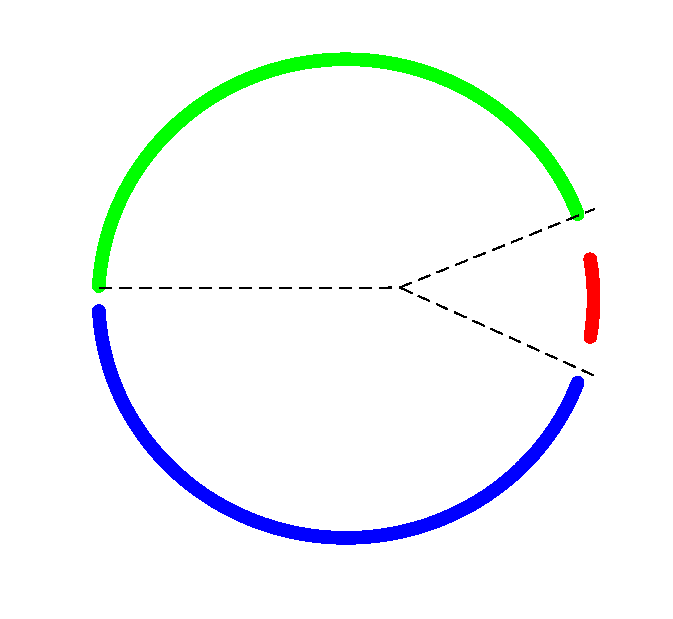
\includegraphics[width=\textwidth, trim={0, 0cm, 0, 0}, clip]{figures/strong_banditron_points}
        \caption{Strongly separable case}
        \end{center}
    \end{subfigure}
    \begin{subfigure}[b]{0.25\textwidth}
        \captionsetup{justification=centering}
        \centering
        \includegraphics[width=\textwidth, trim={0, 0cm, 0, 0}, clip]{figures/weak_banditron_points}
         \caption{Weakly separable case}
    \end{subfigure}
    \captionsetup{justification=centering}
    \caption{\textsc{Banditron}'s final decision boundaries}
     \label{fig:banditron-points}
\end{figure}

\begin{figure}[h!]
    \centering
    \begin{subfigure}[b]{0.25\textwidth}
        \captionsetup{justification=centering}
        \begin{center}
        \includegraphics[width=\textwidth, trim={0, 0cm, 0, 0}, clip]{figures/strong_linear_ova_points}
        \caption{Strongly separable case}
        \end{center}
    \end{subfigure}
    \begin{subfigure}[b]{0.25\textwidth}
        \captionsetup{justification=centering}
        \centering
        \includegraphics[width=\textwidth, trim={0, 0cm, 0, 0}, clip]{figures/weak_linear_ova_points}
         \caption{Weakly separable case}
    \end{subfigure}
    \captionsetup{justification=centering}
    \caption{Algorithm~\ref{algorithm:algorithm-for-strongly-linearly-separable-examples}'s final decision boundaries}
    \label{fig:linearova-points}
\end{figure}
%Our Algorithm with linear kernel (
%To better understand how each algorithm works,
%Our Algorithm with rational kernel (

\begin{figure}[h!]
    \centering
    \begin{subfigure}[b]{0.25\textwidth}
        \captionsetup{justification=centering}
        \begin{center}
        \includegraphics[width=\textwidth, trim={0, 0cm, 0, 0}, clip]{figures/strong_rational_ova_points}
        \caption{Strongly separable case}
        \end{center}
    \end{subfigure}
    \begin{subfigure}[b]{0.25\textwidth}
        \captionsetup{justification=centering}
        \centering
        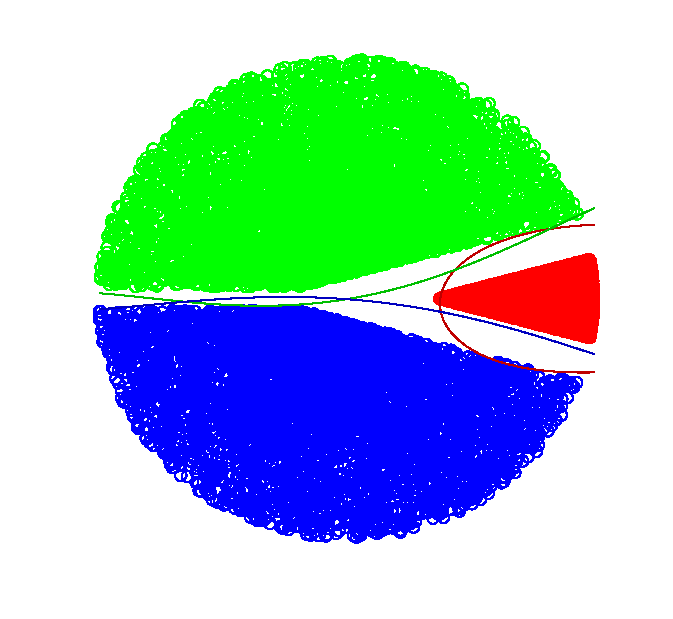
\includegraphics[width=\textwidth, trim={0, 0cm, 0, 0}, clip]{figures/weak_rational_ova_points}
         \caption{Weakly separable case}
    \end{subfigure}
    \captionsetup{justification=centering}
    \caption{Algorithm~\ref{algorithm:kernelized} (with rational kernel)'s final decision boundaries}
    \label{fig:rationalova-points}
\end{figure}

\section{Nearest neighbor algorithm}
\label{section:nearest-neighbor-algorithm}

\begin{algorithm}[H]
\SetAlgoLined
\LinesNumbered
\caption{\textsc{Nearest-Neighbor Algorithm}
\label{algorithm:nearest-neighbor}
}
\textbf{Require:} Number of classes $K$, number of rounds $T$. \\
\textbf{Require:} Inner product space $(V,\ip{\cdot}{\cdot})$. \\
\nl Initialize $S \gets \emptyset$ \\
\nl \For{$t=1,2,\ldots,T$:}{
\nl  \If{$\min_{(x,y) \in S} \norm{x_t - x} \le \gamma$}{
\nl    Find nearest neighbor \\
       \qquad \qquad $(\widetilde{x}, \widetilde{y}) = \argmin_{(x,y) \in S} \norm{x_t - x}$ \\
\nl	  Predict $\widehat{y}_t = \widetilde{y}$
  }
  \Else{
\nl	  Predict $\widehat y_t \sim \text{Uniform}(\{1,2,\dots,K\})$
      \label{line:nearest-neighbor-explore} \\
\nl	  Receive feedback $z_t = \indicator{\widehat{y}_t \neq y_t}$ \\
\nl	  \If{$z_t = 0$}{
\nl      $S \gets S \cup \cbr{(x_t, \widehat{y}_t)}$
    }
  }
}
\end{algorithm}

In this section we analyze \textsc{Nearest-Neighbor Algorithm} shown as
Algorithm~\ref{algorithm:nearest-neighbor}. The algorithm is based on obvious
the idea that under weak linear assumption two examples that are close to each
other must have the same label. Lemma below formalizes this intuition.

\begin{lemma}[Non-separation lemma]
\label{lemma:non-separation-lemma}
Let $(V,\ip{\cdot}{\cdot})$ be a vector space, $K$ be a positive integer and let
$\gamma$ be a positive real number. Suppose $(x_1,y_1), (x_2,y_2), \dots, (x_T,
y_T) \in V \times \{1,2,\dots,K\}$ are labeled examples that are weakly linearly
separable with margin $\gamma$. For $i$, $j$ in $\cbr{1,2,\dots,T}$, if
$\norm{x_i - x_j}_2 \le \gamma$ then $y_i = y_j$.
\end{lemma}

\begin{proof}
Suppose for the sake on contradiction that $y_i \neq y_j$. By
Definition~\ref{definition:linear-separability}, there exists
vectors $w_1, \ldots, w_K$ such that
conditions~\eqref{equation:weak-linear-separability-1}
and~\eqref{equation:weak-linear-separability-2} are satisfied.

Specifically,
\begin{align*}
\ip{w_{y_i} - w_{y_j}}{x_i} & \ge \gamma \; , \\
\ip{w_{y_j} - w_{y_i}}{x_j} & \ge \gamma \; .
\end{align*}
This implies that
$$
\ip{w_{y_i} - w_{y_j}}{x_i - x_j} \ge 2\gamma \; .
$$

On the other hand,
$$
\ip{w_{y_i} - w_{y_j}}{x_i - x_j} \le \norm{w_{y_i} - w_{y_j}} \cdot \norm{x_i - x_j} \le \sqrt{2} \gamma
$$
where the first inequality is from Cauchy-Schwartz inequality, the second
inequality is from that $\norm{w_{y_i} - w_{y_j}} \le \sqrt{2(\norm{w_{y_i}}^2 +
\norm{w_{y_j}}^2)} \leq \sqrt{2}$ and our assumption on $x_i$ and $x_j$.
Therefore, we reach a contradiction.
\end{proof}

We also need to define several notions. A subset $S \subseteq \R^d$ is called a
$\gamma$-packing if for any $x,x' \in S$ such that $x \neq x'$ we have $\norm{x -
x'} > \gamma$. The following lemma is standard. Also recall that $\B(x,R) = \{ x'
\in \R^d ~:~ \norm{x' - x} \le R \}$ denotes the closed ball of radius $R$
centered a point $x$.

\begin{lemma}[Size of $\gamma$-packing]
\label{lemma:size-of-packing}
Let $\gamma$ and $R$ be positive real numbers.
If $S \subseteq \B(\zero,R) \subseteq \R^d$ is a $\gamma$-packing then
$$
|S| \le \left( \frac{2R}{\gamma} + 1 \right)^d \; .
$$
\end{lemma}

\begin{proof}
If $S$ is a $\gamma$-packing then $\{ \B(x,\gamma/2) ~:~ x \in S \}$
is a collection of disjoint balls of radius $\gamma$ that fit into $\B(\zero,R + \gamma/2)$.
Thus,
$$
|S| \cdot \Vol(\B(\zero, \gamma/2)) \le \Vol(\B(\zero,R + \gamma/2))
$$
Hence,
\begin{align*}
|S|
& \le \frac{\Vol(\B(\zero,R + \gamma/2))}{\Vol(\B(\zero, \gamma/2))} \\
& = \left( \frac{R + \gamma/2}{\gamma/2} \right)^d \\
& = \left( \frac{2R}{\gamma} + 1 \right)^d \; .
\end{align*}
\end{proof}

\begin{theorem}[Mistake upper bound for \textsc{Nearest-Neighbor Algorithm}]
\label{theorem:mistake-bound-for-nearest-neighbor-algorithm}
Let $K$ and $d$ be positive integers and let $\gamma,R$ be a positive real
numbers. Suppose $(x_1,y_1), \ldots, (x_T, y_T) \in
\R^d \times \{1,2,\dots,K\}$ are labeled examples that are weakly linearly
separable with margin $\gamma$ and satisfy $\norm{x_1}, \norm{x_2}, \dots,
\norm{x_T} \le R$. Then, the expected number of mistakes made by
Algorithm~\ref{algorithm:nearest-neighbor} is at most
$$
(K-1) \left( \frac{2R}{\gamma} + 1\right)^d \; .
$$
\end{theorem}

\begin{proof}
Let $M$ be the number of mistakes made by the algorithm. Let $b_t$ be the
indicator that line~\ref{line:nearest-neighbor-explore} is executed at timestep
$t$, i.e. we fall into the ``else'' case. Note that if $b_t = 0$, then by
Lemma~\ref{lemma:non-separation-lemma}, the prediction $\widehat{y}_t$ must equal
$y_t$, i.e. $z_t = 0$. Therefore, $M = \sum_{t=1}^T z_t = \sum_{t=1}^T b_t z_t$.
Let $U = \sum_{t=1}^T b_t (1-z_t)$. Clearly, $|S| = U$. Since $S \subseteq \B(\zero, R)$
is a $\gamma$-packing, $U = |S| \le (\frac{2R}{\gamma} + 1)^d$.

Note that when $b_t = 1$, $\widehat{y}_t$ is chosen uniformly at random, we have
$$
\Exp[ z_t ~|~ b_t = 1] = \frac{K-1}{K} \; .
$$
Therefore,
$$
\Exp[M] = \Exp \left[ \sum_{t=1}^T b_t z_t \right] = \frac{K-1}{K} \Exp \left[ \sum_{t=1}^T b_t \right] \; .
$$
On the other hand,
$$
\Exp[U] = \Exp \left[ \sum_{t=1}^T b_t (1-z_t) \right] = \frac 1 K \Exp \left[\sum_{t=1}^T b_t \right] \; .
$$
Therefore,
$$
\Exp[M] = (K-1) \Exp[U] \leq (K-1) \left(\frac{2R}{\gamma} + 1 \right)^d \; .
$$
\end{proof}

\section{NP-hardness of the weak labeling problem}

Any algorithm for the bandit setting collects information in the form of so
called \emph{strongly labeled} and \emph{weakly labeled} examples.
Strongly-labeled examples are those for which we know the class label. Weakly
labeled example is an example for which we know that class label can be anything
except for a particular one class.

A natural strategy for each round is to find vectors $w_1, w_2, \dots, w_K$ that
linearly separate the examples seen in the previous rounds and use the vectors
to predict the label in the next round. More precisely, we want to find both the
vectors $w_1, w_2, \dots, w_K$ and label for each example consistent with its
weak and/or strong labels such that $w_1, w_2, \dots, w_K$ linearly separate the
labeled examples. We show this problem is NP-hard even for $K=3$.

Clearly, the problem is at least as hard as the decision version of the problem
where the goal is to determine if such vectors and labeling exist. We show that
this problem is NP-complete.

We use for $1,2,\dots,K$ for strong labels and $\overline{1}, \overline{2},
\dots, \overline{K}$ for weak labels. We adopt the convention that
$\overline{\overline{i}} = i$ for any positive integer $i$. Formally, the weak
labeling problem can be described as below:
\begin{figure}[H]
\begin{framed}
\begin{center}
    \textbf{Weak Labeling}
\end{center}
\textbf{Given:} Feature-label pairs $(x_1, y_1)$, $(x_2, y_2)$, \dots, $(x_T, y_T)$ in $\{0,1\}^d \times \{1,2,\dots, K, \overline{1}, \overline{2}, \dots, \overline{K}\}$. \\
\textbf{Question:} Do there exist $ w_1, w_2, \dots, w_K \in \R^d$ such that for all $t=1,2,\dots,T$,
\begin{align*}
& y_t \in \{1,2,\dots,K\} \Longrightarrow  \\
& \quad \forall i \in \{1,2,\dots,K\} \setminus \{y_t\} \quad \ip{w_{y_t}}{x_t}  > \ip{w_i}{x_t} \; , \\
& \text{and} \\
& y_t \in \{\overline{1}, \overline{2},\dots, \overline{K}\} \Longrightarrow \\
& \quad \exists i \in \{1,2,\dots,K\} \quad \ip{w_i}{x_t} > \ip{w_{\overline{y_t}}}{x_t} \; ?
\end{align*}
\end{framed}
\end{figure}

The hardness proof is based on a reduction from the set splitting problem, which
is proven to be NP-complete by Lovasz \cite{Garey-Johnson-1979}, to our weak
labeling problem. The reduction is adapted from \cite{Blum-Rivest-1993}.
\begin{figure}[H]
\begin{framed}
\begin{center}
    \textbf{Set Splitting}
\end{center}
\textbf{Given:} A finite set $S$ and a collection $C$ of subsets $c_i$ of $S$. \\
\textbf{Question:} Do there exist disjoint sets $S_1$ and $S_2$ such that $S_1 \cup S_2 = S$ and $\forall i, c_i\not\subseteq S_1$ or $c_i\not\subseteq S_2$?
\end{framed}
\end{figure}

Below we show the reduction. Suppose we are given an instance of the set
splitting problem
\begin{align*}
S & = \{1, 2, \dots, N\} \; , \\
C & = \{c_1, c_2, \dots, c_M\} \; .
\end{align*}

We create the weak labeling instance as follows. Let $d=N+1$ and $K=3$.
Define $\zero$ as the zero vector $(0,\dots,0)\in \R^N$ and $\e_i$ as the
$i$-th standard vector $(0,\dots, 1, \dots, 0)\in \R^N$). Then we include all
the following feature-label pairs:
\begin{itemize}
\item Type 1: $(x,y)=((\zero,1), 3)$,
\item Type 2: $(x,y)=((\e_i,1), \overline{3})$ for all $i \in \{1,2,\dots,N\}$,
\item Type 3: $(x,y)=\left(\left(\sum_{i\in c_j} \e_i, 1\right), 3\right)$ for all $j \in \{1,2,\dots,M\}$.
\end{itemize}

For example, if we have $S=\{1,2,3\}$, $C=\{c_1, c_2\}$, $c_1 = \{1,2\}$,
$c_2=\{2,3\}$, then we create the weak labeling sample set as:
\begin{multline*}
\{
((0,0,0,1),3), ((1,0,0,1),\overline{3}), ((0,1,0,1),\overline{3}), \\
((0,0,1,1),\overline{3}), ((1,1,0,1),3), ((0,1,1,1),3)
\} \; .
\end{multline*}
The following lemma shows that answering this weak labeling problem is
equivalent to answering the original set splitting problem.

\begin{lemma}
Any instance of the set splitting problem is a YES instance if and only if the
corresponding instance of the weak labeling problem (as described above) is a
YES instance.
\end{lemma}

\begin{proof}
$(\Longrightarrow)$ Let $S_1, S_2$ be the solution of the set splitting problem. Define
$$
w_1 = \left(a_1, a_2, \cdots, a_N, -\frac{1}{2}\right),
$$
where for all $i \in \{1,2,\dots,N\}$, $a_i=1$ if $i\in S_1$ and $a_i=-N$ if
$i\notin S_1$. Similarly, define
$$
w_2 = \left(b_1, b_2, \cdots, b_N, -\frac{1}{2}\right),
$$
where for all $i \in \{1,2,\dots,N\}$, $b_i=1$ if $i \in S_2$ and $b_i=-N$ if
$i\notin S_2$. Finally, define
$$
w_3 = (0,0,\cdots, 0),
$$
the zero vector. To see this is a solution for the weak labeling problem, we
verify separately for Type 1-3 samples defined above. For Type 1 sample, we have
$$
\ip{w_3}{x} = 0 > -\frac{1}{2} = \ip{w_1}{x}=\ip{w_2}{x}.
$$
For a Type 2 sample that corresponds to index $i$, we have either $i\in S_1$ or
$i\in S_2$ because $S_1\cup S_2 = \{1,2,\dots,N\}$ is guaranteed. Thus, either
$a_i=1$ or $b_i=1$. If $a_i=1$ is the case, then
$$
\ip{w_1}{x} = a_i - \frac{1}{2} = \frac{1}{2} > 0 = \ip{w_3}{x};
$$
similarly if $b_i=1$, we have $\ip{w_2}{x}>\ip{w_3}{x}$. \\ For a Type 3 sample
that corresponds to index $j$, Since $c_j \not\subset S_1$, there exists some
$i'\in c_j$ and $i'\notin S_1$. Thus we have $x_{i'}=1$, $a_{i'}=-N$, and
therefore
\begin{align*}
\ip{w_1}{x}
& = a_{i'}x_{i'} + \sum_{i\in \{1,2,\dots,N\} \setminus \{i'\}} a_ix_i - \frac{1}{2} \\
& \le -N + (N-1)-\frac{1}{2} \\
& < 0 = \ip{w_3}{x} \; .
\end{align*}
Because $c_j \not\subset S_2$ also holds, we also have
$\ip{w_2}{x}<\ip{w_3}{x}$. This direction is therefore proved. \\
\ \\
$(\Longleftarrow)$ Given the solution $w_1, w_2, w_3$ of the weak labeling problem, we define
\begin{align*}
S_1 &= \left\{i \in \{1,2,\dots,n\} ~:~ \ip{w_1-w_3}{(\e_i, 1)} > 0 \right\}, \\
S_2 &= \left\{i \in \{1,2,\dots,n\} ~:~ \ip{w_2-w_3}{(\e_i, 1)} > 0 \text{\ and\ } i\notin S_1 \right\}.
\end{align*}
It is not hard to see $S_1 \cap S_2 = \emptyset$ and $S_1\cup S_2 =
\{1,2,\dots,N\}$. The former is because $S_2$ only includes elements that are
not in $S_1$. For the latter, note that $(\e_i, 1)$ is the feature vector for
Type 2 samples. Because Type 2 samples all have label $\overline{3}$, for any $i
\in \{1,2,\dots,N\}$, one of the following must hold: $\ip{w_1-w_3}{(\e_i,
1)}>0$ or $\ip{w_2-w_3}{(\e_i, 1)}>0$. This implies $i\in S_1$ or $i\in S_2$.

Now we show $\forall j$, $c_j \not\subset S_1$ and $c_j \not\subset S_2$ by
contraction. Assume there exists some $j$ such that $c_j \subset S_1$. By our
definition of $S_1$, we have $\ip{w_1-w_3}{(\e_i, 1)} > 0$ for all $i\in c_j$.
Therefore,
\begin{align*}
\sum_{i\in c_j} \ip{w_1-w_3}{\left(\e_i, 1\right)}
& = \ip{w_1-w_3}{\left(\sum_{i\in c_j} \e_i, |c_j|\right)}  \\
& > 0.
\end{align*}
Because Type 1 sample has label $3$, we also have
$$
\ip{w_1-w_3}{\left(\zero, 1\right)} < 0.
$$
Combining the above two inequalities, we get
\begin{align*}
& \ip{w_1-w_3}{\left(\sum_{i\in c_j}\e_i, 1\right)} \\
& = \ip{w_1-w_3}{\left(\sum_{i\in c_j}\e_i, |c_j|\right)}  \\
& \qquad - (|c_j|-1)\ip{w_1-w_3}{\left(\zero, 1\right)} \\
& > 0 \; .
\end{align*}
Note that $\left(\sum_{i\in c_j}\e_i, 1\right)$ is a feature vector for Type 3
samples. Thus the above inequality contradicts that Type 3 samples have label 3.
Therefore, $c_j \not\subset S_1$. If we assume there exists some $c_j \subset
S_2$, same arguments apply and also lead to contradiction.
\end{proof}

\section{Mistake lower bound for ignorant algorithms}
\label{section:mistake-lower-bound-for-ignorant-algorithms}

In this section, we prove a mistake lower bound for a family of algorithms
called \textit{ignorant algorithms}. Ignorant algorithms ignore the examples on
which they make mistakes. This assumption seems strong, but as we will explain
below, it is actually natural, and several recently proposed bandit
classification algorithms that achieve $\sqrt{T}$ regret bounds belong to
this family, e.g., SOBA~\citep{Beygelzimer-Orabona-Zhang-2017},
OBAMA~\citep{Foster-Kale-Luo-Mohri-Sridharan-2018}. Also,
\textsc{Nearest-Neighbor Algorithm} (Algorithm~\ref{algorithm:nearest-neighbor})
presented in Appendix~\ref{section:nearest-neighbor-algorithm} is an ignorant
algorithm.

Under the assumption that the examples lie in in the unit ball of $\R^d$ and are
weakly linearly separable with margin $\gamma$, we show that any ignorant
algorithm must make at least $\Omega \left( \left(\frac{1}{160 \gamma}\right)^{(d-2)/4} \right)$
mistakes in the worst case. In other words, an algorithm that achieves a better
mistake bound cannot ignore examples on which it makes a mistake and it must
make a meaningful update on such examples.

To formally define ignorant algorithms, we define the conditional distribution
from which an algorithm draws its predictions. Formally, given an algorithm
$\calA$ and an adversarial strategy, we define
\begin{multline*}
p_t(y|x) = \\
\Pr[y_t = y ~|~ (x_1, y_1), (x_2, y_2) \dots, (x_{t-1}, y_{t-1}), x_t = x] \; .
\end{multline*}
In other words, in any round $t$, conditioned on the past $t-1$ rounds, the
algorithm $\calA$ chooses $y_t$ from probability distribution $p_t(\cdot|x_t)$.
Formally, $p_t$ is a function $p:\{1,2,\dots,K\} \times \R^d \to [0,1]$
such that $\sum_{y=1}^K p_t(y|x) = 1$ for any $x \in \R^d$.

\begin{definition}[Ignorant algorithm]
An algorithm $\calA$ for \textsc{Online Multiclass Linear Classification with
Bandit Feedback} is called \emph{ignorant} if for every $t=1,2,\dots,T$,
$p_t$ is determined solely by the sequence
$(x_{a_1}, y_{a_1}), (x_{a_2}, y_{a_2}), \dots, (x_{a_n}, y_{a_n})$
in the rounds $1 \le a_1 < a_2 < \dots < a_n < t$ in which
the algorithm makes a correct prediction.
\end{definition}

An equivalent definition of an ignorant algorithm is that the memory state of
the algorithm does not change after it makes a mistake. Equivalently,
the memory state of an ignorant algorithm is completely determined
by the sequence of labeled examples on which it made correct prediction.

To explain the definition, consider an ignorant algorithm $\calA$. Suppose that
on a sequence of examples $(x_1, y_1), (x_2, y_2), \dots, (x_{t-1}, y_{t-1})$
generated by some adversary the algorthm $\calA$ makes correct predictions in
rounds $a_1, a_2, \dots, a_n$ where $1 \le a_1 < a_2 < \dots < a_n < t$ and
errors on rounds $\{1,2,\dots,t-1\} \setminus \{a_1, a_2, \dots, a_n\}$. Suppose
that on another sequence of examples $(x_1', y_1'), (x_2', y_2'), \dots,
(x_{s-1}', y_{s-1}')$ generated by another adversary the algorithm $\calA$ makes
correct predictions in rounds $b_1, b_2, \dots, b_n$ where $1 \le b_1 < b_2 <
\dots < b_n < s$ and errors on rounds $\{1,2,\dots,s-1\} \setminus \{b_1, b_2,
\dots, b_n\}$. Futhermore, suppose
\begin{align*}
(x_{a_1}, y_{a_1}) &= (x'_{b_1}, y'_{b_1}) \; , \\
(x_{a_2}, y_{a_2}) &= (x'_{b_2}, y'_{b_2}) \; , \\
\vdots \\
(x_{a_n}, y_{a_n}) &= (x'_{b_2}, y'_{b_n}) \; .
\end{align*}
Then, the definition
\begin{multline*}
\Pr[y_t = y ~|~ (x_1, y_1), (x_2, y_2) \dots, (x_{t-1}, y_{t-1}), x_t = x] = \\
\Pr[y_t' = y ~|~ (x_1', y_1'), (x_2', y_2') \dots, (x_{t-1}', y_{t-1}'), x_t' = x] \; .
\end{multline*}
Note that the sequences $(x_1, y_1)$, $(x_2, y_2)$, $\dots$, $(x_{t-1},
y_{t-1})$ and $(x_1', y_1')$, $(x_2', y_2')$, $\dots$, $(x_{s-1}', y_{s-1}')$
might have different lengths and and $\calA$ might error in different sets of
rounds. As a special case, if an ignorant algorithm makes a mistake in round $t$
then $p_{t+1}=p_t$.

Our main result is the following lower bound on the expected number of mistakes
for ignorant algorithms.

\begin{theorem}[Mistake lower bound for ignorant algorithms]
\label{theorem:ignorant-lower-bound}
Let $\gamma \in (0,1)$ and let $d$ be a positive integer. Suppose $\calA$ is an
ignorant algorithm for \textsc{Online Multiclass Linear Classification with
Bandit Feedback}. There exists $T$ and an adversary that sequentially chooses
labeled examples $(x_1, y_1), (x_2, y_2), \dots, (x_T, y_T) \in \R^d\times
\{1,2\}$ such that the examples are strongly linearly separable with magin
$\gamma$ and $\norm{x_1}, \norm{x_2}, \dots, \norm{x_T} \le 1$, and the expected
number of mistakes made by $\calA$ is at least
$$
\frac{1}{10} \left(\frac{1}{160\gamma}\right)^{\frac{d-2}{4}} \; .
$$
\end{theorem}

Before proving the theorem, we need the following lemma.

\begin{lemma}
\label{lemma:embed_d_gamma}
Let $\gamma \in (0,\frac{1}{160})$, let $d$ be a positive integer and let $N = (\frac{1}{2\sqrt{40\gamma}})^{d-2}$.
There exist vectors $u_1, u_2, \dots, u_N, v_1, v_2, \dots, v_N \in \R^d$ such that for all $i, j \in \{1,2,\dots,N\}$,
\begin{align*}
\norm{u_i} & \le 1 \; , \\
\norm{v_j} & \le 1 \; , \\
\ip{u_i}{v_j} & \ge \gamma & & \text{if $i=j$,} \\
\ip{u_i}{v_j} & \le -\gamma & & \text{if $i \neq j$.}
\end{align*}
\end{lemma}

\begin{proof}
By Lemma 6 of~\citet{Long-1995}, there exists vectors $z_1, z_2, \dots, z_N \in
\R^{d-1}$ such that $\norm{z_1} = \norm{z_2} = \dots = \norm{z_N} = 1$ and the
angle between the vectors is $\measuredangle(z_i, z_j) \ge \sqrt{40 \gamma}$ for
$i \neq j$, $i,j \in \{1,2,\dots,N\}$. Since $\cos\theta \le 1-\theta^2/5$ for
any $\theta \in [-\pi,\pi]$, this implies that
\begin{align*}
\ip{z_i}{z_j} &= 1 && \text{if $i = j$,} \\
\ip{z_i}{z_j} &\le 1 - 8\gamma && \text{if $i \neq j$.}
\end{align*}

Define $v_i = (\frac{1}{2} z_i, \frac{1}{2})$, and $u_i = (\frac{1}{2} z_i,
-\frac{1}{2}(1-4\gamma))$ for all $i \in \{1,2,\dots,N\}$. It can be easily
checked that for all $i$, $\norm{v_i} \le 1$ and $\norm{u_i} \le 1$.
Additionally,
$$
\ip{u_i}{v_j} = \frac{1}{4} \ip{z_i}{z_j} - \frac {1-4\gamma} 4 \; .
$$
Thus,
\begin{align*}
\ip{u_i}{v_j} &\ge \gamma && \text{if $i=j$,} \\
\ip{u_i}{v_j} &\le -\gamma && \text{if $i \neq j$.}
\end{align*}
\end{proof}

\begin{proof}
We consider the strategy for the adversary described in
Algorithm~\ref{algorithm:adversary-strategy}.

\begin{algorithm}
\caption{\textsc{Adversary's strategy}}
\label{algorithm:adversary-strategy}
\textbf{Define} $T=N$ and $v_1, v_2, \dots, v_N$ as in Lemma~\ref{lemma:embed_d_gamma}.\\
\textbf{Define} $q_0=\frac{1}{\sqrt{T}}$. \\
\textbf{Initialize} $\textsc{phase}= 1$. \\
\For{$t=1,2,\dots,T$}{
    \If{$\textsc{phase}=1$}{
       \If{$p_t(1|v_t)\ge 1-q_0$}{
          $(x_t, y_t)\leftarrow (v_t, 1)$
        }
       \Else{
          $(x_t, y_t)\leftarrow (v_t, 2)$ \\
          $\textsc{phase}\leftarrow 2$
       }
    }
    \Else{
         $(x_t, y_t)\leftarrow (x_{t-1}, y_{t-1})$
    }
}
\end{algorithm}

Define the indicators
\begin{align*}
A_t &= \indicator{\forall \tau\le t, p_\tau(1|x_\tau)<1-q_0} \\
B_t &= \indicator{\exists \tau\le t, p_\tau(1|x_\tau)\ge 1-q_0
 \text{\ and\ } \forall s\in[\tau,t), \widehat y_s \neq y_s}.
\end{align*}
Then we have
\begin{align}
& \mathbf{E}\left[\sum_{t=1}^{T} \indicator{\widehat y_t\neq y_t}\right] \nonumber \\
& \ge \mathbf{E}\left[\sum_{t=1}^T \indicator{\widehat y_t\neq y_t}A_t\right] \nonumber \\
& \qquad + \mathbf{E}\left[\sum_{t=1}^T \indicator{\widehat y_t\neq y_t}B_t\right] \nonumber \\
& = \mathbf{E}\left[\sum_{t=1}^T \mathbf{E}_t\left[\indicator{\widehat y_t\neq y_t}A_t\right]\right] + \mathbf{E}\left[\sum_{t=1}^T B_{t+1}\right] \nonumber \\
& \ge \mathbf{E}\left[\sum_{t=1}^T q_0 A_t\right] + \mathbf{E}\left[\sum_{t=1}^T B_{t+1}\right],
\label{equation:mistake_lower_bound_temp}
\end{align}
where in the first inequality we use the fact that $A_t$ and $B_t$ cannot be $1$
simultaneously; in the equality, we use $B_{t+1}=B_t\indicator{\widehat y_t\neq
y_t}$ by $B_t$'s definition; in the last inequality we use the fact that when
$t\le N$ and $A_t=1$, it must be $y_t=1$ and $\Pr[\widehat
y_t=y_t]=p_t(1|x_t)<1-q_0$. Now, denote $T_1 = \argmin_{\tau} \{
p_\tau(1|x_\tau) \ge 1-q_0 \}$ (if such $\tau$ does not exist or is larger than
$T$, we simply let $T_1=T+1$). Then $A_t=1$ for all $t\le
T_1-1$.

Note that $B_{T_1}=1$, and for $t \ge T_1$ the adversary will switch to
``$\textsc{phase}=2$'' and has $y_t=2$. Therefore,
$\Exp[B_{t+1}=0|B_{t}=1]=\Pr[\widehat y_t=y_t~|~B_t=1] = \Pr[\widehat
y_t=2|B_t=1].$ Note that when $B_t=1$, by definition there exists a $\tau\le t$
with $p_\tau(1|x_\tau)\ge 1-q_0$, and the algorithm all makes mistakes at $\tau,
\tau+1, \ldots, t$. Since the algorithm is ignorant, and when
$\textsc{phase}=2$, the features all remain the same, we have
$p_t(1|x_t)=p_{t-1}(1|x_{t-1})=\cdots=p_\tau(1|x_\tau)\ge 1-q_0$. Thus we can
further upper bound $\Exp[B_{t+1}=0|B_{t}=1]$ by $\Pr[\widehat y_t=2|B_t=1]\leq
q_0$. Thus the second term in \eqref{equation:mistake_lower_bound_temp} can be
calculated as

\begin{align*}
\mathbf{E}\left[\sum_{t=1}^T B_{t+1}\right]
& \ge \mathbf{E}\left[\sum_{t=T_1}^T (1-q_0)^{t-T_1+1} \right] \\
& = \frac{1-q_0}{q_0}\mathbf{E}\left[1-(1-q_0)^{T - T_1 + 1}\right] \; .
\end{align*}
Combining \eqref{equation:mistake_lower_bound_temp} and the above inequalities, we get
\begin{multline}
\label{equation:mistake_lower_bound_temp2}
\mathbf{E} \left[\sum_{t=1}^T \indicator{\widehat y_t\neq y_t}\right] \ge
\\ \mathbf{E}\left[q_0(T_1-1)+\frac{1-q_0}{q_0}\left(1-(1-q_0)^{T-T_1+1}\right)\right].
\end{multline}
In the case $T_1\ge \frac{1}{2}T + 1$, the right-hand side of
\eqref{equation:mistake_lower_bound_temp2} is lower bounded by
$\frac{1}{2}q_0 T = \frac{1}{2} \sqrt{T}$. In the case
$T_1< \frac{1}{2}T+1$, it is lower bounded by
\begin{align*}
& \frac{1-q_0}{q_0}\left(1-(1-q_0)^{\frac{1}{2}T}\right) \\
& = \frac{1-q_0}{q_0}\left(1-(1-q_0)^{\frac{1}{2q_0^2}}\right) \\
& \ge \frac{1-\frac{1}{\sqrt{2}}}{q_0}\left(1-\frac{1}{\sqrt{e}}\right) \\
& \ge \frac{1}{10} \sqrt{T} \; .
\end{align*}

Observe that in phase 1, the labels are equal to $1$ and in phase 2 the labels
are equal to $2$. Let $t$ be the round in which the switch happens. (If it never
happens, define $t=T+1$.) Note that $(x_t, y_t)=(x_{t+1}, y_{t+1})= \dots =
(x_T, y_T) = (v_t, 2)$. Consider the vectors $u_1, u_2, \dots, u_N$ as defined
in Lemma~\ref{lemma:embed_d_gamma} We claim that $w_1=-u_t/2$ and $w_2=u_t/2$
satisfy the conditions of strong linear separabaility.

Clearly $\norm{w_1}^2 + \norm{w_2}^2 \le (\norm{w_1} + \norm{w_2})^2 \le
(\frac{1}{2} + \frac{1}{2})^2 \le 1$. By Lemma~\ref{lemma:embed_d_gamma}, we
have $\ip{w_2/2}{x_s} = \ip{u_t/2}{v_t} \ge \gamma/2, \forall s \ge t$ and
$\ip{w_2/2}{x_s} = \ip{u_t/2}{v_s} \le - \gamma/2$ for all $s<t$. Similarly,
$\ip{w_1/2}{x_s} \le -\gamma/2$ for all $s \ge t$ and $\ip{w_1/2}{x_s} \ge
\gamma/2$ for all $s < t$. Thus, the examples are strongly separable with margin
$\gamma$.
\end{proof}


\end{document}
